\makeatletter
%\newcommand{\rmnum}[1]{\romannumeral #1 }
%\newcommand{\Rmnum}[1]{\expandafter\@slowromancap\romannumeral #1@}
\makeatother
\ifpdf
\graphicspath{{Results/ResultsFigs/PNG/}{Results/ResultsFigs/PDF/}{Results/ResultsFigs/}}
\else
\graphicspath{{Results/ResultsFigs/EPS/}{Results/ResultsFigs/}}
\fi

\chapter{Coherence Results and Evaluation}
\label{coherence_eval}
	In this chapter, I compare the performance of BERI coherence models using a multi-threaded benchmark suite. The directory-based model is used as a baseline to evaluate the time-based coherence designs. Single-threaded applications are not generally affected by coherence, however, the peculiar behaviour of time-based coherence may result in some performance penalties. Drawbacks of the coherence model are analysed by testing single-threaded applications available on FreeBSD.
	
	The performance of a given coherence model is evaluated based on the test execution time. I have also added a range of hardware counters to the BERI L1 caches. These counters display statistics of the cache, and cache coherence behaviour. Data extracted from the counters is also used to estimate the coherence communication energy.

\section{Splash-2 Benchmarks}
	I have used the Splash-2 benchmark suite to evaluate parallel performance, sourced from \cite{splash2_0,splash2_1,splash2_2}. This suite was selected for several reasons: it is written in C which is supported by CHERI LLVM (C++ is currently unavailable), widely used in memory architecture research, and the benchmarks are well understood.

	The Splash-2 suite contains a number of applications based around scientific parallel compute. Most tests in the suite heavily rely on efficient shared memory block transfer. Several tests from the suite were selected for primary evaluation of the dual-core BERI designs. The selected tests are sufficiently diverse and display many problem flavours. 

	%\subsection{Test Behaviour}
	Benchmarks have been compiled using the CHERI LLVM compiler to run on the FreeBSD OS (Section \ref{freebsd_setup}). The produced binaries can be executed directly under FreeBSD on our various BERI hardware designs on FPGA (Section \ref{fpga_implementation}). The benchmark characteristics and resource usage have been documented by Woo et al. \cite{Woo95}, Bienia et al. \cite{Bienia08}, and Barrow-Williams et al. \cite{Barrow-Williams09}. This information is briefly summarised in this section; it will be referenced in further sections to explain the  observed behaviour. The benchmark details and default test setting are listed below:
			
		\label{test_settings_splash}
		\begin{description}
			\item[LU Contiguous (LU+)] This benchmark uses dense linear algebra to factorise a matrix. The matrix is subdivided into smaller arrays and allocated contiguously in local memory, allowing processors to exploit temporal locality. Inter-array communication causes synchronisation delays, up to 25\% of the total execution time. 
			This test is evaluated using a matrix size of 512.
			
			\item[LU Non-Contiguous (LU--)] In this version of LU, the matrix is factored into a two-dimensional array, preventing contiguous memory allocation. Since the LU tests are somewhat similar, I evaluate this version using a smaller matrix size of 128.

			\item[Water N-Squared (Water-N)] This application calculates the behaviour of water molecules. Particle computations are stored locally and accumulated into a shared copy at the end, reducing synchronisation. Evaluated using a problem size of 512.

			\item[Water Contiguous (Water-S)] This benchmark is similar to Water N-Squared, but uses a more efficient computation algorithm. The problem is split into a uniform grid of cells; molecular movement between cell boundaries requires shared communication. Evaluated using a problem size of 512.
			
			\item[Radix] This application is an iterative integer sorting algorithm. The problem is subdivided, allowing each processor to generate a local histogram.
			A global histogram is formed using the local results. This histogram is split and distributed for the next iteration, resulting in bursty communication traffic. The working set of this algorithm is not precisely defined and may lead to cache capacity misses. Evaluated using a Radix size of 1024.
			
			\item[FFT Small and Large (FFT-S and FFT-L)] This algorithm is widely used in signal processing. Data is subdivided into matrices, partitioned in favour of local cache access and optimised for low interprocessor communication. This test may cause shared memory penalties if the private caches cannot accommodate all local data. Since there is only one version of FFT, the benchmark was evaluated with two configurations, FFT-Small (complex doubles: 1024; bytes/line: 16) and FFT-Large (complex doubles: 16384; bytes/line: 64)
			
			\item[FMM Small and Large (FMM-S and FMM-L)] This application simulates a system of particles. Interactions occur in a two-dimensional format. FMM displays an unstructured communication pattern, subject to potential false sharing. The benchmark is evaluated with two sets of input parameters; FMM-Small (particles: 256) and FMM-Large (particles: 2048).
			
			\item[Ocean Contiguous (Ocean+)] This test simulates the flow of ocean currents. 
			Data is arranged in multidimensional arrays. One of the dimension specifies an owner processor. Data is contiguously allocated to each processor, enhancing locality properties, and reducing false sharing.
			Higher problem sizes are likely to result in substantial capacity and conflict misses, thus, testing the memory system design. Evaluated using a grid size of 258.
			
			\item[Ocean Non-Contiguous (Ocean--)] The data is partitioned in two-dimensional arrays and cannot be contiguously allocated in memory. The two Ocean tests are very diverse, using different styles of inter-core communication. This version exhibits high proportion of shared memory traffic, up to 50\% of all memory communication. Evaluated using a grid size of 258.
		\end{description}
		
		
		
	\section{Effects of Time-outs on Performance}
		In this section I test the BERI time-based coherence model using a range of static cache line time-outs, in order to determine the best average performer. All time-based models are compared against a baseline set by the BERI directory coherence scheme. Benchmarks are tested using a software thread count of 2, allowing minimal parallel behaviour necessary for a dual-core system. All other test setting are left as default (Section \ref{test_settings_splash}).
		
		Each Splash test has been executed a minimum of 10 times. Error bars represent the standard deviation for each test. All data is normalised against the BERI directory coherence model. Each tested time-based coherence model uses fixed time-out value, indicating the lifespan of a cache line in cycles. For example, in time-based (1,000), a cache line will be valid for one thousand cycles. If this line is accessed by the pipeline beyond that limit, it will self-invalidate. Figures \ref{splash_combined}, \ref{splash_combined_ratio}, and \ref{splash_combined_inv_ratio} show the obtained results. 
		
		\paragraph{Figure \ref{splash_combined}} shows the mean execution time per benchmark per hardware model. The coherence models displayed are arranged in the following order, from left to right:
			\begin{enumerate}
				\item Directory Coherence: Dual-core BERI using directory coherence with short-tags optimisation.
				\item Time-Based Coherence (1,000,000): Dual-core BERI using self-invalidating private data caches with a line time-out of one million cycles.
				\item Time-Based Coherence (100,000): Identical architecture to the model above but using a time-out of one hundred thousand cycles.
				\item Time-Based Coherence (10,000): Identical architecture to the model above but using a time-out of ten thousand cycles.
				\item Time-Based Coherence (1,000): Identical architecture to the model above but using a time-out of one thousand cycles.
			\end{enumerate}

		\begin{figure}[!b]
		\centering 
			\makebox{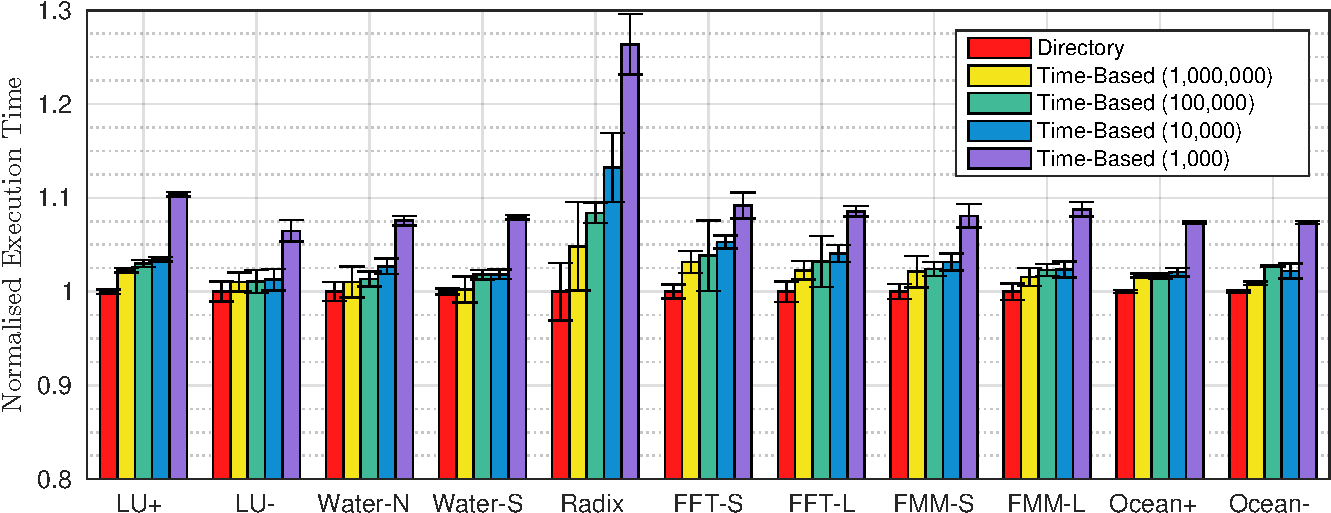
\includegraphics[width=\textwidth,height=\textheight,keepaspectratio,angle=0]{splash_combined_freebsd}}
			\caption[Splash-2 execution time, 2 software threads]{Splash-2 execution time, 2 software threads (\textit{Lower is better})} 
			\label{splash_combined}
		\end{figure}

		\paragraph{Figure \ref{splash_combined_ratio}} shows the hit/miss ratio for each coherence model. Ratios are constructed using the mean values of total hits and misses accumulated by the cache hardware counters. Note that counter values are extracted from each processor core and then combined to form one global result.
		
		\paragraph{Figure \ref{splash_combined_inv_ratio}} shows metrics specific to the architectures of directory-based and time-based models, they are not directly comparable. In the directory case, the total number of invalidation messages generated by the directory is compared to the number of messages matching a sharer cache entry (coherence address is compared with the short-tags). Matching entries are referred to as invalidate-hits, all remaining messages are false invalidates (they do not invalidate any cache lines). 
		
		In the time-based models, the number of cache misses triggered by self-invalidation are compared to the total number of cache misses.

		Directory-based coherence shows a strong overall performance. However, the best performing time-based model is within 3\% of the directory results. In 9 of the 11 tests, directory coherence shows a statistically significant performance advantage. In the remaining 2 tests (Water-N and Water-S), results displayed by the time-based model are within the standard deviation. The algorithms used in these tests require less synchronisation which is beneficial to the time-based model.
		
		Across the full range of time-based model tests, time-based (1,000,000) shows the best overall performance, supporting the general caching philosophy of exploiting spacial and temporal data locality.
		The execution time of each time-based model is directly proportional to the selected time-out value. 
		For most tests, all time-based designs fall within a 10\% range of the directory results.
		In all tests other than Radix, the models with a time-out between 10,000 and 1,000,000 cycles show a very similar execution time, often in a 2\% range.
		
		Overall, directory coherence shows a strong cache behaviour with most tests achieving a hit ratio of 92\% or more.
		False-invalidates occur when shared data is loaded and then used for some operations but never updated.
		The L2 cache maintains a strict inclusion policy, so when shared data is evicted, coherence messages are sent to all sharers. False messaging could be reduced by optimising the coherence mechanism to exploit typical memory sharing patterns \cite{Cuesta11,Cuesta13}.

		The time-based (1,000,000) model achieves better hit ratios than other time-based variants. In most tests its hit ratio is within 1--3\% of that shown by the directory. The time-based model actually shows a better hit ratio for LU-Contiguous. For the same test the directory shows its best ratio of true invalidates, indicating very efficient synchronisation. The LU test highlights the characteristics of a coherence mechanism, as high cache hit ratios do not necessarily result in a superior overall performance.
		This issue will be elaborated further in this chapter.
		
		In Figure \ref{splash_combined_ratio}, comparing (d) and (b), the time-out is increased by a factor of 100, but the hit ratio only improves by $\sim$4\%. The worst performing time-based (1,000) shows an average slowdown between 8\% and 25\%. If we ignore the slowest model, all other time-based versions fall within 3\% of the directory performance, for this configuration of benchmarks. 
		
		On the whole the slowest model demonstrates that these benchmarks require more than 1,000 cycles to perform a set of operations before synchronising or moving to a different block of data. The cost of time-counter roll-overs is also evident as memory is blocked for longer. Individual benchmark behaviour will be elaborated in further sections.

		\clearpage
		\begin{figure}[!h]
		\centering 
			\makebox{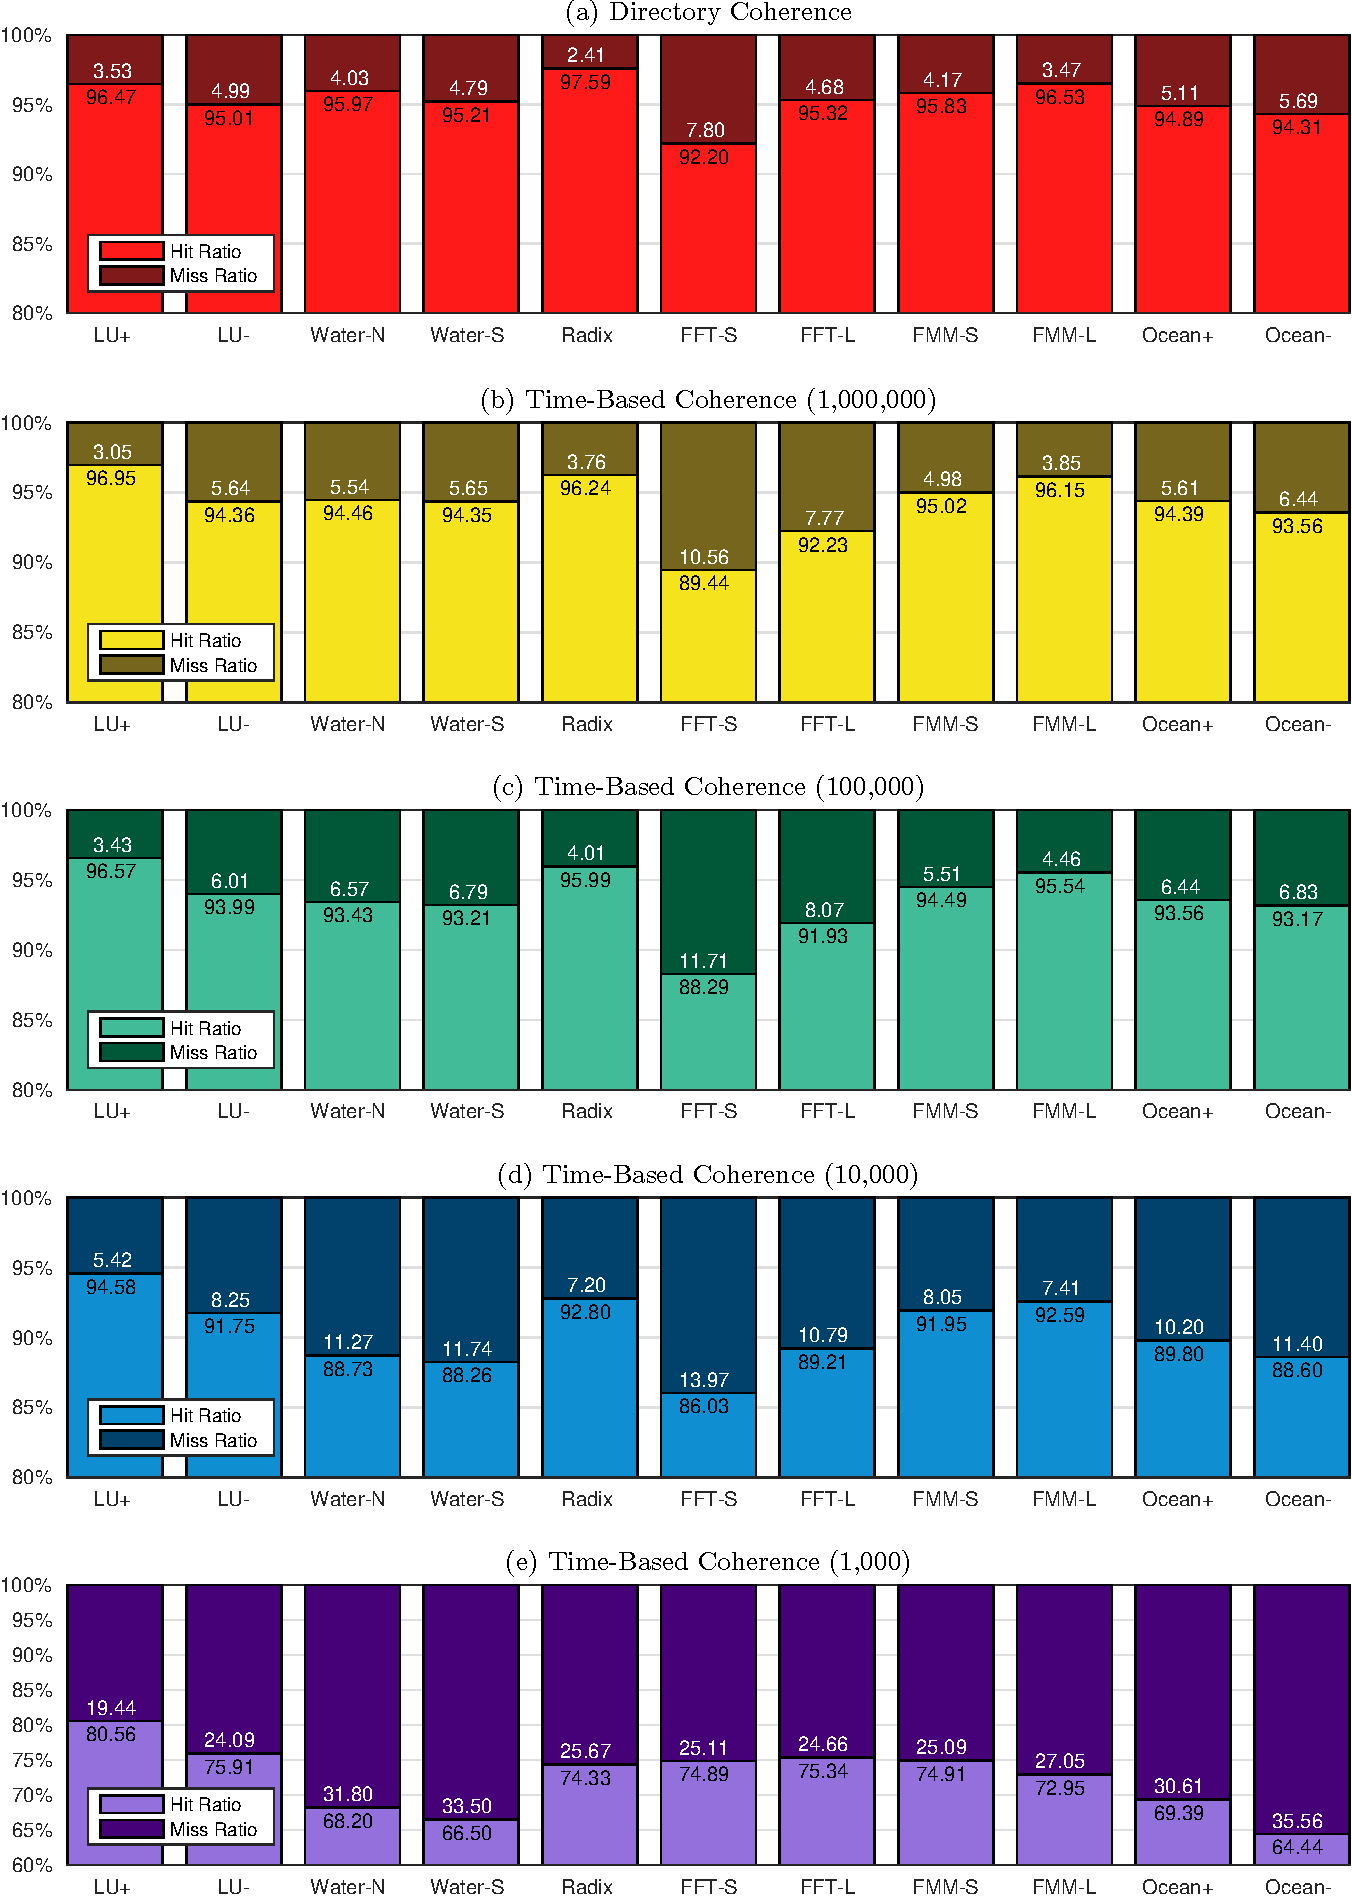
\includegraphics[width=\textwidth,height=\textheight,keepaspectratio,angle=0]{splash_combined_ratio}}
			\caption[Splash-2 hit/miss ratios]{Splash-2 hit/miss ratios. Charts (b), (c), and (d) show a similar pattern for the range of benchmarks (\textit{Note: A wider y-axis is used in (e). Charts show a ratio between total cache hits and misses, the total number of memory accesses are affected by the coherence mechanism, and may differ})} 
			\label{splash_combined_ratio}
		\end{figure}
		
		\begin{figure}[!h]
		\centering 
			\makebox{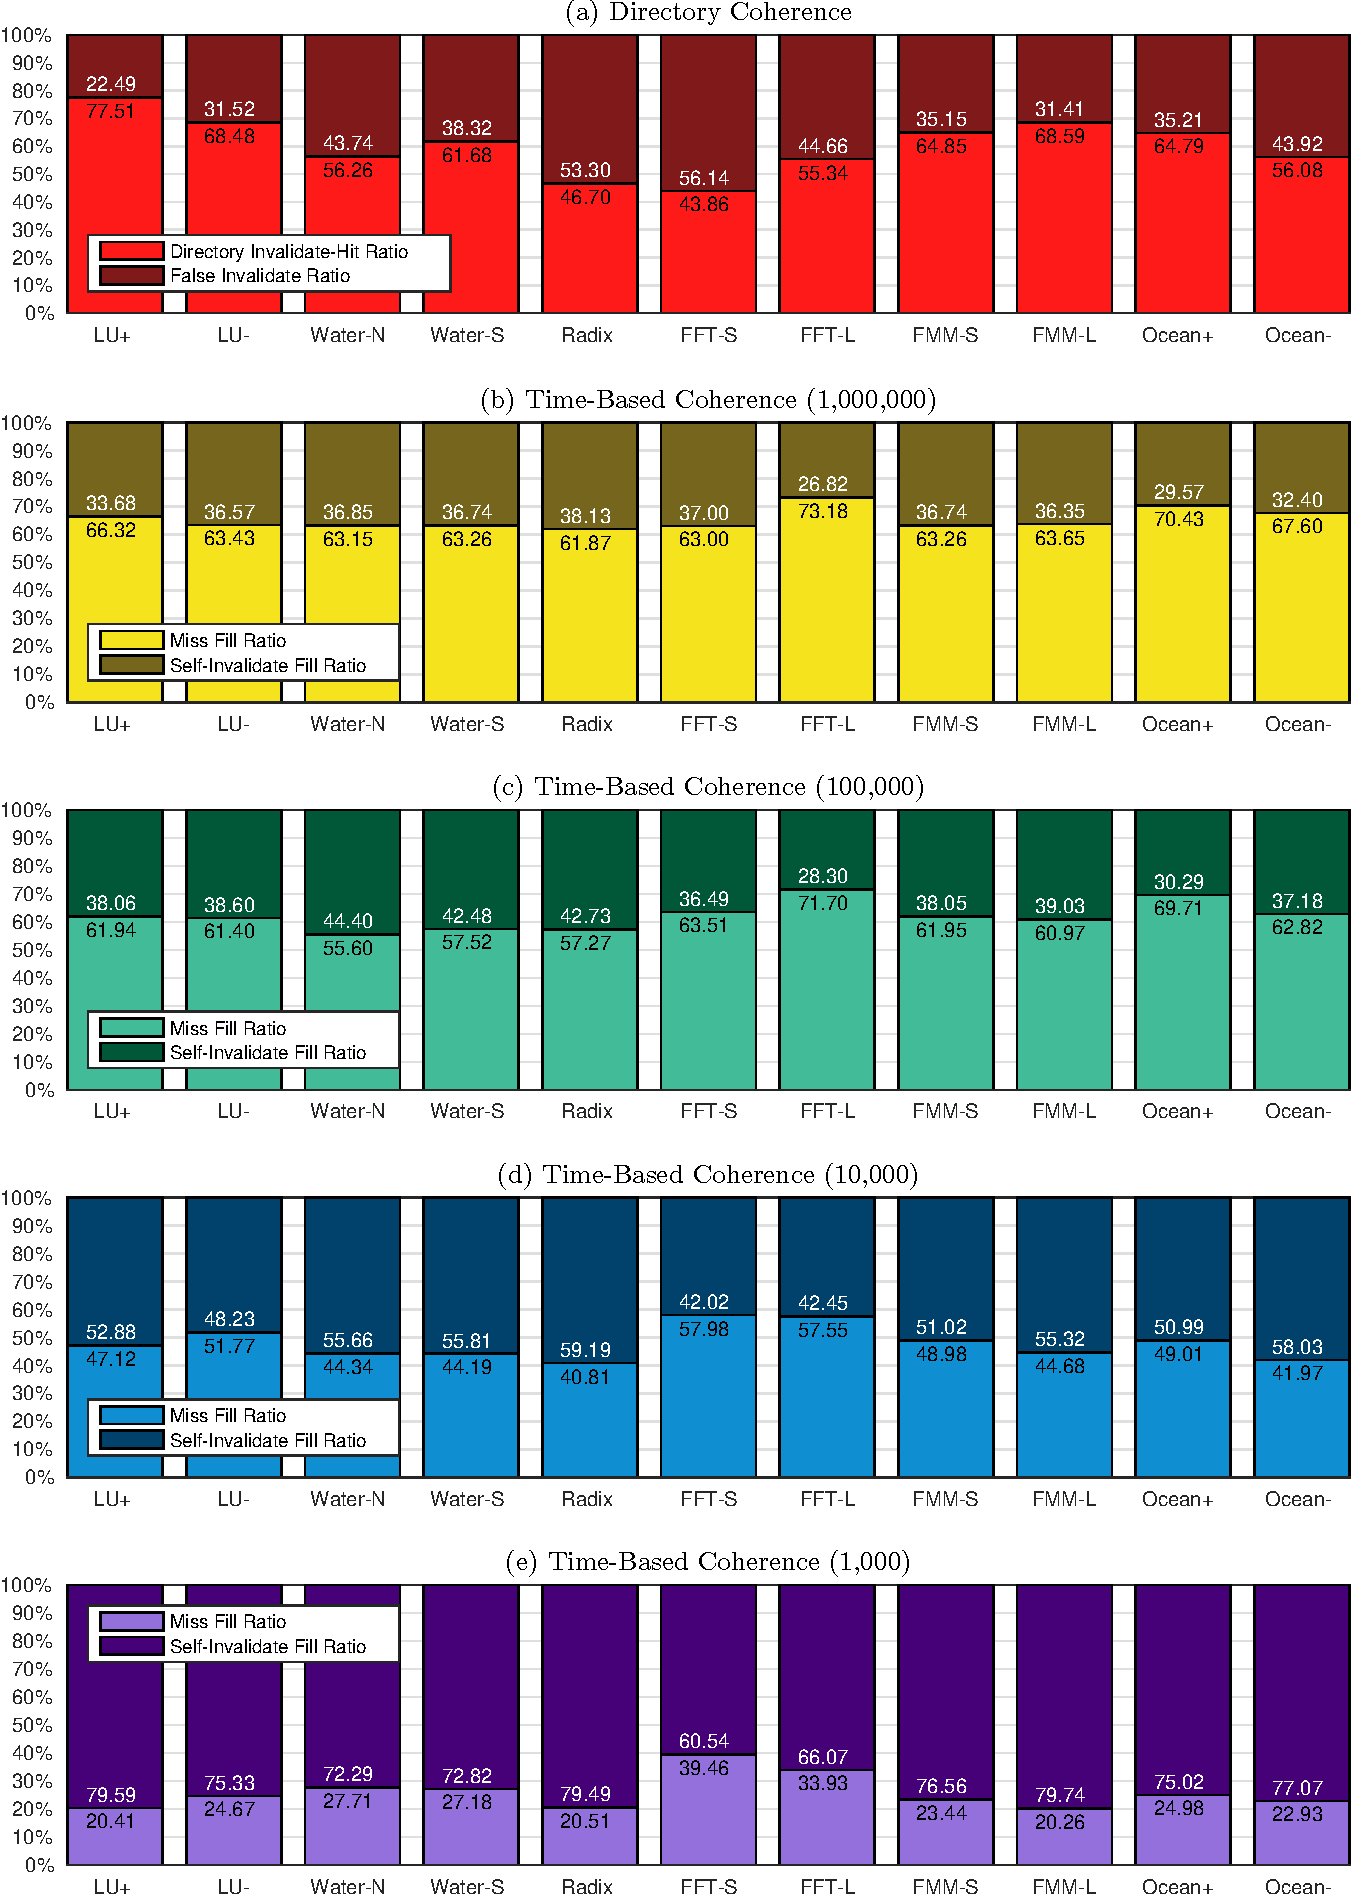
\includegraphics[width=\textwidth,height=\textheight,keepaspectratio,angle=0]{splash_combined_inv_ratio}}
			\caption[Splash-2 directory-invalidate and self-invalidate ratios]{Splash-2 directory-invalidate and self-invalidate ratios. Across the range of benchmarks, all time-based models show a similar self-invalidation pattern. (\textit{Note: Chart (a) shows invalidate messages issues by the directory in the L2 cache, (b,c,d,e) show tag-time-stamp expiry within the L1 data caches})} 
			\label{splash_combined_inv_ratio}
		\end{figure}
	
\clearpage
	\section{Optimising Time-Based Coherence}
		Prior evaluation has shown that the time-based model benefits from a longer cache time-out; fewer time-counter roll-overs. In this set of tests I evaluate cache optimisations that could improve performance.
		The benchmarks were previously tested using a software thread count of 2, in this set of tests the thread count has been increased to 16. It is a good balance between the minimum and maximum number of software threads (1--64) supported by Splash-2 tests. Results are presented in Figures \ref{splash_16thread_freebsd}, \ref{splash_16thread_hit_ratio}, and \ref{splash_16thread_inv_ratio}.
		
		Earlier tests have shown that time-based (1,000,000) model displayed the best performance of all compared time-based models. In this section I compare three BERI models: directory-based coherence, time-based (1,000,000), and time-based (1,000,000) with the polling detection [PD] (introduced in Section \ref{polling_detection_mechanism}).
		
		The time-based (1,000,000) standard model shows an improvement over the previous evaluation in Figure \ref{splash_combined} (especially LU+, Water-N, FFT-L, FMM-L, and Ocean-). The directory is affected by the increased thread count, showing a greater number of false invalidates and a marginally lower hit rate, approximately 1\%. 
		
		Time-based PD shows a more balanced performance as compared to the standard version, outperforming it outright in 5 tests. In the remaining 6 tests, the PD model shows a comparable or lower standard deviation. 
		
		The LU benchmark imposes large synchronisation overheads (Section \ref{test_settings_splash}). For 16 software threads, the time-based model shows an improved LU Contiguous execution, however, the LU Non-Contiguous results are weaker. The LU Contiguous algorithm exploits cache temporal locality by subdividing the test dataset. The Non-Contiguous version uses a coarse grained approach, which results in more communication.
		
		
		\begin{figure}[!h]
		\centering 
			\makebox{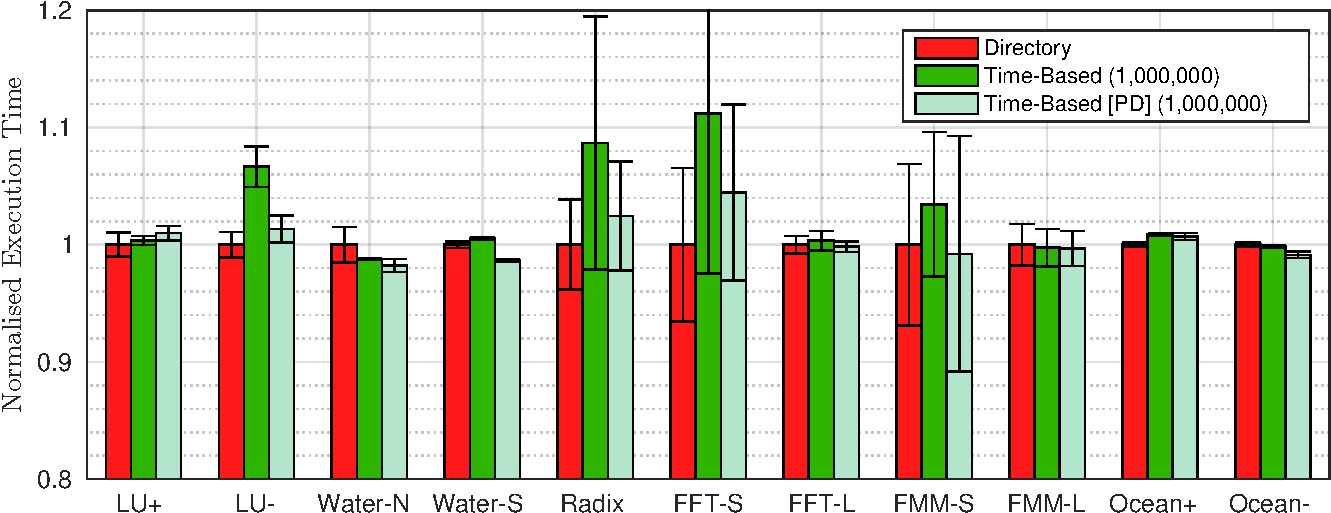
\includegraphics[width=\textwidth,height=\textheight,keepaspectratio,angle=0]{splash_16thread_freebsd}}
			\caption[Splash-2 execution time, 16 software threads]{Splash-2 execution time, 16 software threads (\textit{Lower is better})} 
			\label{splash_16thread_freebsd}
		\end{figure}
		%\vspace{-5mm}

\clearpage
		\begin{figure}[!h]
		\centering 
			\makebox{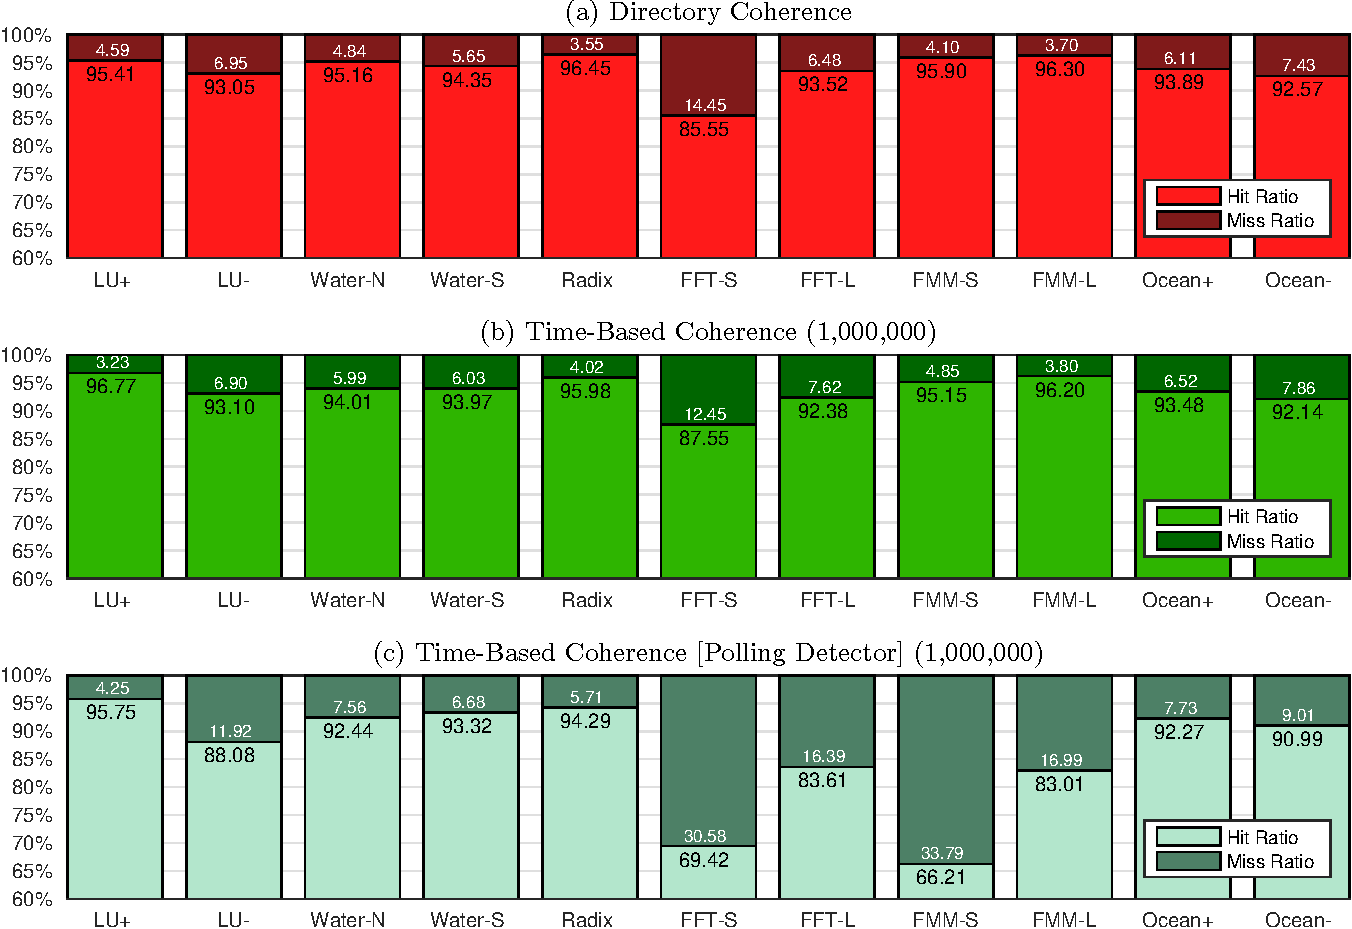
\includegraphics[width=\textwidth,height=\textheight,keepaspectratio]{splash_16thread_hit_ratio}}
			\vspace{-7mm}
			\caption{Splash-2 hit/miss ratios, 16 threads} 
			\label{splash_16thread_hit_ratio}
		\end{figure}
%\vspace{-5mm}
		\begin{figure}[!h]
		\centering 
			\makebox{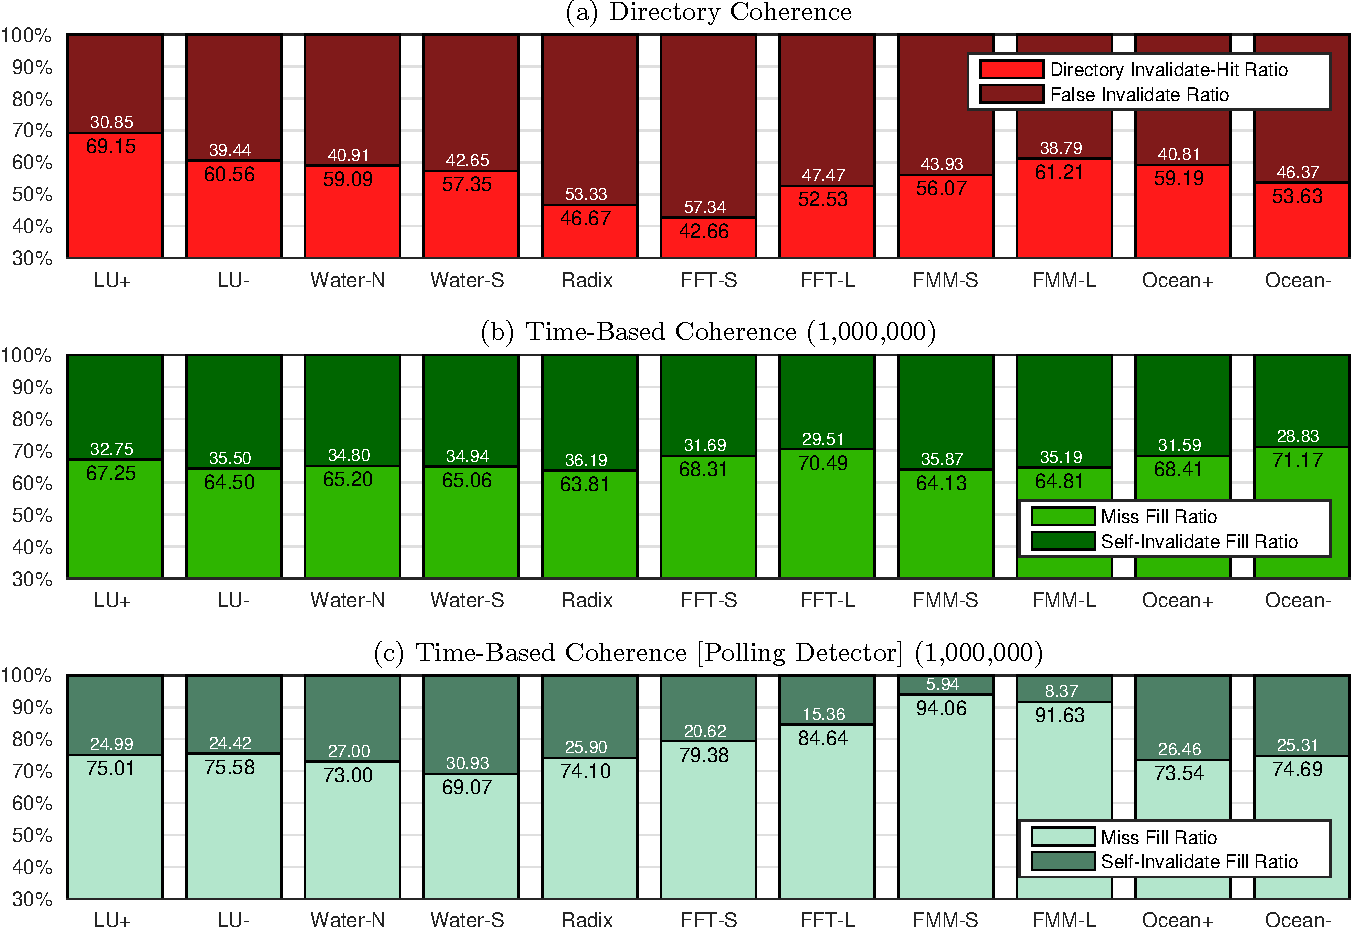
\includegraphics[width=\textwidth,height=\textheight,keepaspectratio]{splash_16thread_inv_ratio}}
			\vspace{-7mm}
			\caption{Splash-2 directory-invalidate and self-invalidate ratios, 16 threads} 
			\label{splash_16thread_inv_ratio}
		\end{figure}
\vspace{-10mm}

\clearpage
		The time-based PD version shows a much lower hit rate for LU Non-Contiguous, which results in a performance degradation. Note that the PD version shows lower hit rates for all benchmarks, but a better self-invalidation ratio, since misses due to polling detection are not counted. 
		
		The Water benchmarks are designed to reduce overall coherence communication and synchronisation. Both time-based models respond positively to this test, with the PD model showing a $\sim$2\% improvement over the directory. 
		
		The Radix test uses a bursty communication pattern and a constantly varying dataset size. Both factors negatively affect the time-based model as time-counter roll-overs are more frequent than in other tests. A larger tag-time-stamp is likely to improve performance. The PD model responds much better to Radix than the default design.
		
		FFT-Small forces more communication due to a smaller a dataset and partitions, whereas FFT-Large will cause shared memory penalties due to L1 capacity misses. The latter allows time-based coherence to show a better baseline relative performance. The small version of this test severely penalises the time-based model, despite showing a better hit rate than the directory. The PD model shows a much lower hit rate, but also fewer self-invalidates indicating polling detection.
		
		For FMM Small and Large, the PD model shows its best self-invalidation ratio, but a weaker overall hit ratio due to polling detection. The directory design suffers due to the coherence communication overheads imposed by this test.
		
		For both Ocean benchmarks the time-based designs perform better than the 2 thread evaluation. A significant proportion of memory references are shared and all models demonstrate a similar behaviour and cache hit ratios.
		

	\section{Extended Splash-2 Comparison}
		In this section the performance of time-based coherence is analysed using a range of Splash-2 test parameters. Five tests are used in this evaluation: both LU, Radix, and both Ocean tests. These tests should provide sufficient evidence to understand the coherence behaviour. In each test, two main parameters are varied: dataset block size and software thread count. Figures \ref{splash_extended_polling} and \ref{splash_extended_standard} show the obtained results. The directory results are shown as a flat baseline.
		
		The time-based PD model consistently outperforms the standard version. It is also clear that an increase in block size (reduction in synchronisation) yields better performance. Execution time rises with an increase in software thread count. Note that in the Ocean Contiguous evaluation, the grid size value of 10 is insufficient for testing 32 and 64 threads.
		
		This experiment shows that the polling detection mechanism is still useful in parallel applications that largely depend on locks and barriers. These results also confirm my predictions of the drawbacks of the current time-based model. They can be reduced by either increasing the TTS size or using a different technique for triggering time-outs.

		\paragraph{Figure \ref{splash_extended_standard} --} Time-based coherence 1,000,000.
		\begin{description}
			\item [(a) LU Contiguous] An increase in thread size negatively affects the coherence behaviour as more synchronisation is necessary. However, a larger workload compensates for this overhead and produces a close to baseline performance. A small dataset is severely affected by an increase in thread count.
			\item [(b) LU Non-Contiguous] This test displays a similar behaviour to that shown in (a), but in this test the performance impact of a small dataset is lower. Also, a similar response to software threads is observed.
			\item [(c) Radix] This test has shown the largest performance overheads for the time-based model in all previous evaluations. The coherence model responds negatively to both the dataset size and thread count. For 64 threads and a 1024 Radix, the performance is almost 50\% worse than the directory equivalent. 
			\item [(d) Ocean Contiguous] Similar to the tests discussed above, this Ocean benchmark displays a higher coherence overhead for smaller datasets. The overheads for software threads are reasonable for up to 8--16 threads, but rapidly increase for 32 or more. The time-based model actually performs better than the directory for the default test grid size of 258. 
			\item [(e) Ocean Non-Contiguous] The results are similar to those shown in (d), however, this test shows better scalability for 32 and 64 threads.
		\end{description}
		
		\paragraph{Figure \ref{splash_extended_polling} --} Time-based coherence 1,000,000 with memory polling detection. The individual test behaviour is almost identical to the standard time-based model, but the execution time for each test variant in lower. All of the tests execute faster for smaller datasets. The execution time for Radix and Ocean tests running 32--64 threads is almost 25\% better than the standard model.
		
		This test demonstrates that the time-based model can be significantly improved through optimisations such as the polling detection mechanism. While the performance for small datasets is poor relative to the directory, memory hungry tests can benefit from this model.

\clearpage
		\begin{figure}[!h]
		\centering 
			\makebox{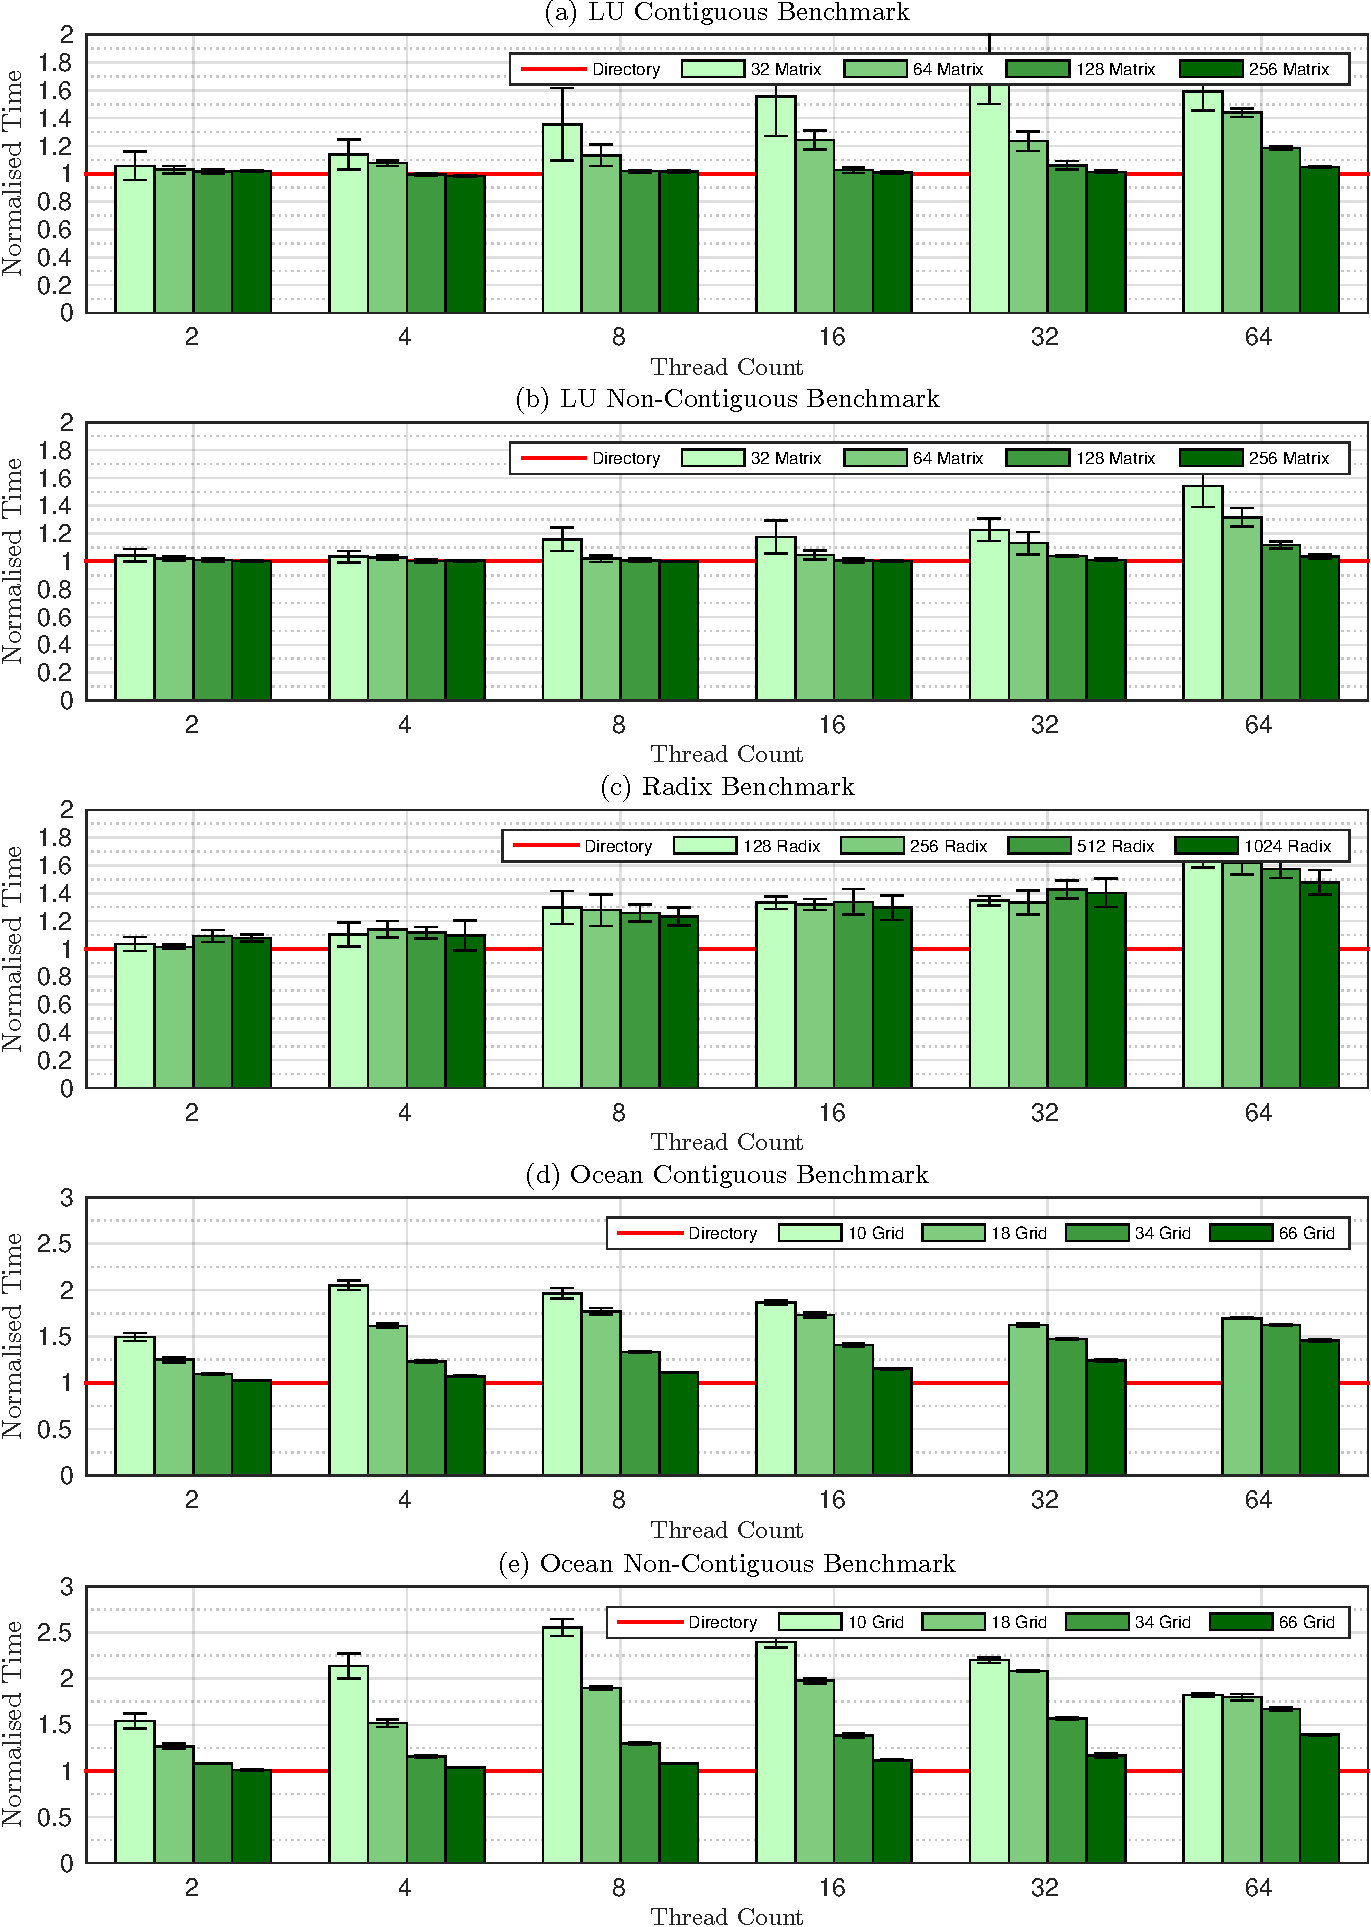
\includegraphics[width=\textwidth,height=\textheight,keepaspectratio,angle=0]{splash_extended_standard}}
			\caption[Splash-2 extended benchmarks, part 1]{Splash-2 extended benchmarks, time-based coherence 1,000,000 (\textit{Note: Each chart shows the total execution time taken per evaluation parameter, normalised using the mean baseline established by the BERI Directory model. The thread count represents the number of software threads spawned by each benchmark})} 
			\label{splash_extended_standard}
		\end{figure}
		%\vspace{-5mm}

		\begin{figure}[!h]
		\centering 
			\makebox{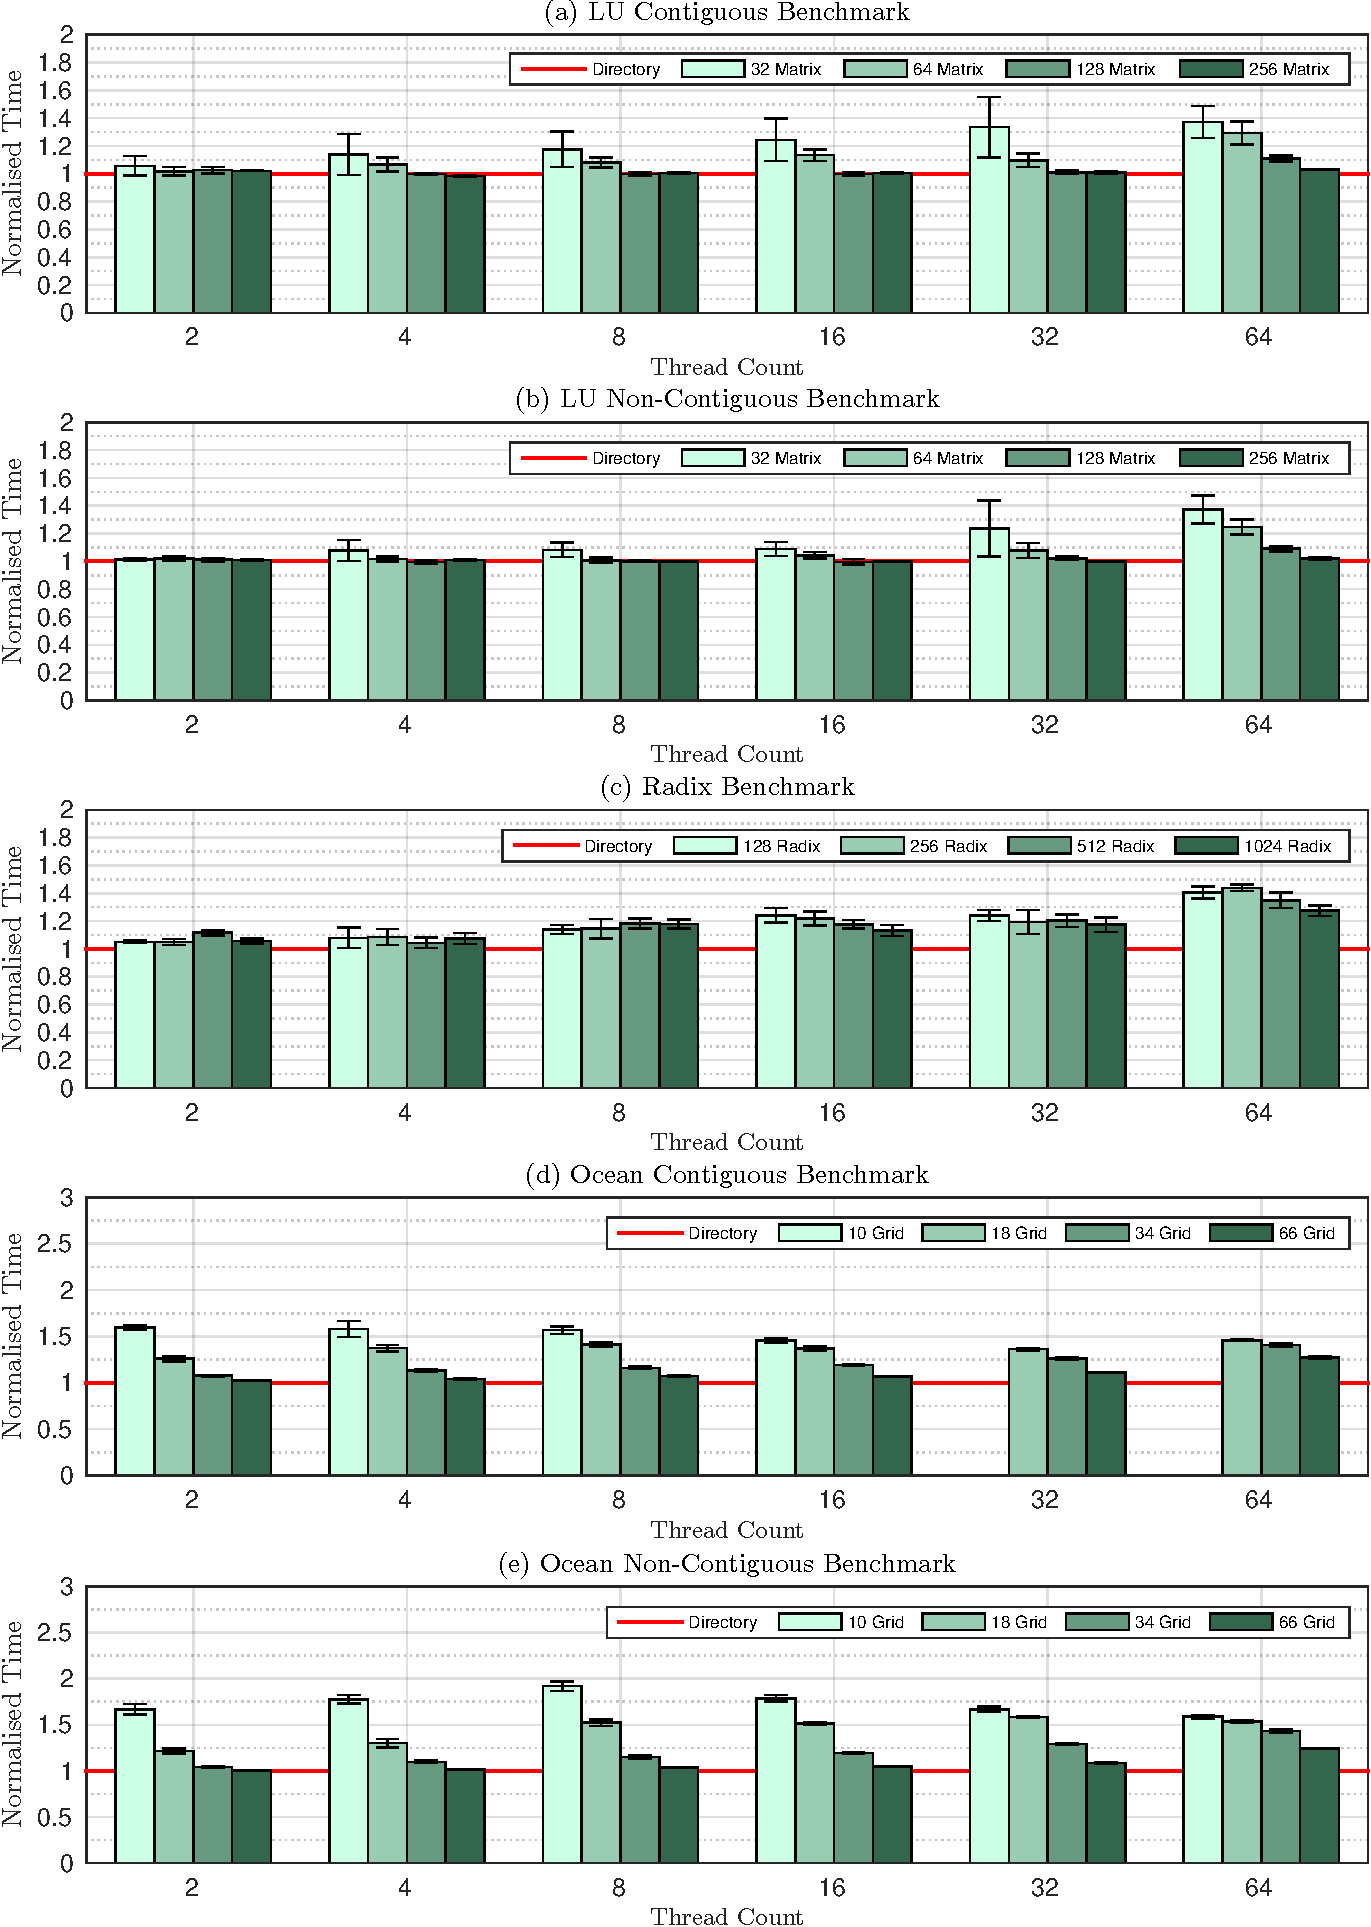
\includegraphics[width=\textwidth,height=\textheight,keepaspectratio,angle=0]{splash_extended_polling}}
			\caption[Splash-2 extended benchmarks, part 2]{Splash-2 extended benchmarks, time-based coherence 1,000,000 with memory polling detection (\textit{Note: Each chart is compared against the mean execution time of the BERI Directory model, same baseline as shown in Figure \ref{splash_extended_standard}. The Ocean benchmarks are displayed using a different scale})} 
			\label{splash_extended_polling}
		\end{figure}
		%\vspace{-5mm}	
		

\clearpage
	\section{Effects of Cache Size on Performance}
		In this section I evaluate the performance variations arising from changing the cache size; the cache design is not altered. 
		I am interested in understanding whether an increase in either to L1 or L2 cache size will adversely effect the performance of the BERI coherence mechanisms, time-based in particular. 
		One disadvantage of the current version of the time-based coherence model is that time-counter roll-overs cause cache reinitialisation; effectively a slow cache flush. This property has not shown a significant disadvantage in the default tests, however, an increase in the L1 size will increase the overheads of reinitialisation; a larger cache leads to a longer blocking time.
		
		The directory model may also be affected by the increase in either the L1 or L2 size, since a bigger L1 will force greater L2 inclusion and potentially a higher capacity miss rate. A larger L2 will likely improve the outcome, as capacity misses will reduce, thus reducing the number of forced coherence messages. Larger L1's may actually have a negative effect as they will cache more data, so the directory will likely need to track more shared data, leading to higher coherence messaging due to L2 capacity misses.
		
		I am also testing a design where both L1 and L2 are increased in size. Note that only the L1 data cache is increased and the L1 instruction cache is kept constant throughout. A total of 8 models are tested using the same benchmark settings as shown in Figure \ref{splash_16thread_freebsd}, 16 software threads. The BERI directory and BERI time-based polling detection (1,000,000) are compared to three variants: double L1 size, double L2 size, and double L1 and L2 caches.

		\begin{figure}[!h]
		\centering 
			\makebox{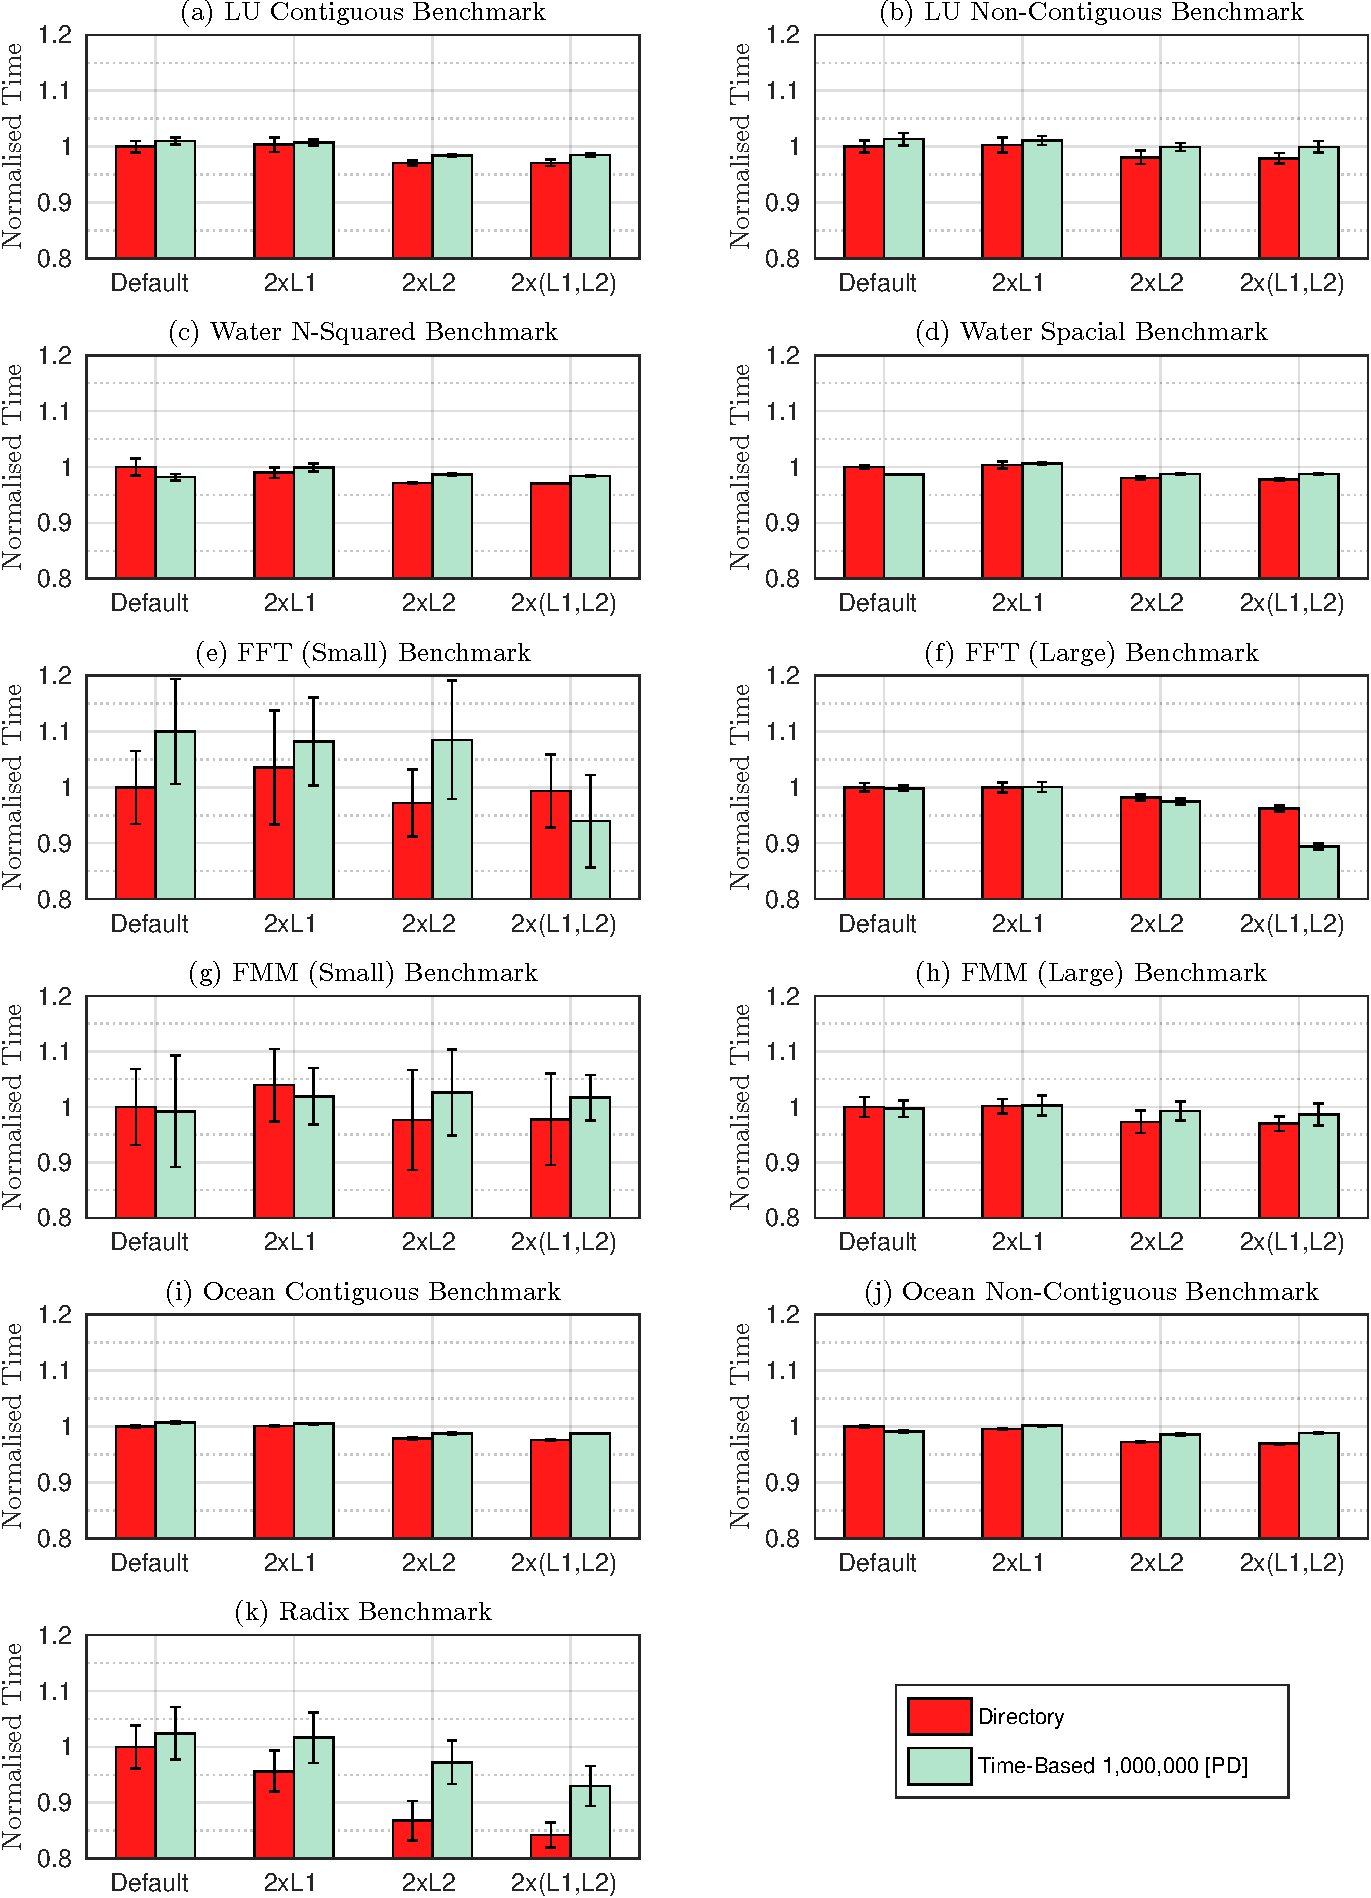
\includegraphics[width=\textwidth,height=\textheight,keepaspectratio,angle=0]{splash_big_cache_full}}
			\vspace{-3mm}
			\caption[Splash-2 cache size vs. coherence]{Splash-2 cache size vs. coherence (\textit{Note: Each test is evaluated using the default benchmark parameters and 16 threads, as stated in previous sections. All tests results are normalised relative to the default directory evaluation})} 
			\label{splash_big_cache_full}
		\end{figure}

		\begin{description}
			\item [(a) LU Contiguous] The directory and time-based models show a similar response in the default and 2xL1 tests. Doubling the L1 caches does not benefit either model. Both models show an improvement in the 2xL2 and 2x(L1,L2) tests, however, the directory gains a bigger advantage. This is likely due to a reduction in invalidates as shared line evictions are reduced in the L2 cache.
			\item [(b) LU Non-Contiguous] Both models show a similar pattern to that demonstrated in (a). Neither model is penalised by the changes in cache size. The time-based model improves with an increase in the L2 cache size but the directory shows a better improvement.
			\item [(c) Water N-Squared] In this test the directory model shows a steady improvement with a size increase in any of the caches. The time-based model holds an advantage in the default case but shows weaker performance once the L1 cache size is increased, likely due to a larger time-counter roll-over overhead. An increase in the L2 size improves over the 2xL1 case, however, none of the results quite match the default case.
			\item [(d) Water Spacial] This test demonstrates an almost identical behaviour to that of Water N-Squared.
			\item [(e) FFT-Small] In this test the directory model is penalised whenever the L1 cache size is increased. More data is privately cached which then results in L2 capacity misses and additional coherence messaging. The best performance is shown when only the L2 size is increased, supporting the reasons mentioned above. The time-based model shows some improvement over the default in both the 2xL1 and 2xL2 tests. This test produces a wide range of results, as illustrated by the standard deviation. Interestingly the combination of a larger L1 and L2 results in a significant improvement.
			\item [(f) FFT-Large] The relative performance of the time-based model is much better than in (e). A larger data block size causes fewer synchronisations, benefiting the time-based model. The directory response to an increased L1 is less dramatic; a larger data block size reduces the number of capacity misses, as blocks are not constantly replaced in the L2.
			\item [(g) FMM-Small] The directory is heavily penalised in the 2xL1 case, similar reasons to (e). A larger L2 cache rectifies the performance drop. The time-based model appears to be penalised when either the L1 or the L2 are increased, however, the block size of this test is small so the behaviour is unpredictable due to frequent synchronisation operations. Note the standard deviation for both models, the results show a significant overlap for every cache configuration.
			\item [(h) FMM-Large] Similar to the transition in FFT from Small to Large, this test also shows more stable results as compared to (g). The directory only improves when the L2 cache is increased. The time-based model shows a similar behaviour but loses out to the directory for both 2xL2 and 2x(L1,L2) tests.
			\item [(i) Ocean Contiguous] This test is likely to cause substantial capacity and conflict misses, as a result both coherence models show an improvement when the L2 cache size is increased. The overall performance improvement of the directory model is marginally better.
			\item [(j) Ocean Non-Contiguous] In this test the time-based model is better in the default case, however, it is penalised by an increase in L1 size. This is visible in both 2xL1 and 2x(L1,L2) tests. The test generates a large number of shared memory references and fast coherence communication benefits the directory model.
			\item [(k) Radix] This test shows the most drastic change in relative performance between the two models. It also confirms the previous observations of this test, which have shown that the time-based model suffers serious overheads. On every iteration the sorting algorithm builds local data clusters which are later merged and redistributed. This generates bursty synchronisation traffic that penalises the time-based model. However, both models show a significant improvement with an increase in any cache size, more than any other test in this set-up. This further proves that more cache spaces allows local Radix histograms to be stored and immediately reused, while capacity misses would result in frequent requests to main memory which are costly.
		\end{description}


%\clearpage
\section{Evaluating FreeBSD Commands}
	\label{results_polling}
	
	The purpose of these tests is to demonstrate that the time-based coherence model does not adversely affect single-threaded performance. Some common command line applications available in FreeBSD have been tested. These commands are single threaded, so instead of testing shared memory interactions, we observe any shortcomings or pitfalls in the behaviour of time-based coherence. Note that the OS is concurrently executed and some scheduler interference is expected. Each test run is sampled a minimum of 10 times.
	
	Communication centric coherence schemes should have little or no effect on single threaded applications as no shared memory interactions occur, hence, no coherence messaging is required. The strict inclusion policy required in the BERI directory coherence scheme could still impact the overall performance, as accurate directory tracking may produce false coherence messages.
	
	The automatic self-invalidations in the time-based coherence scheme will likely affect the performance of these applications. In fact, self-invalidates are shown to be useful and necessary for the given set of applications. I have developed the memory polling detection (PD) scheme specifically due to the preliminary evaluation of these applications. The effect is most significant in the CP test where the standard and PD versions show a dramatic performance difference, the standard version is up to 4 times slower than the PD model. This will be discussed in more detail in Section \ref{results_cp}.
	
	The tests results show that the time-based coherence model does affect single threaded programs as hypothesised, however, the models with PD or lower time-out values, usually fall within 10\% of the directory results. The advantages of directory coherence are evident in these examples and further improvements in polling detection could benefit the time-based model. Identifying sharing patters, producer-consumer relations, and other memory behaviour profiling is often used for optimising coherence schemes \cite{Byrd99,Lilja93,Sanchez12,Cuesta11}.

%\clearpage
	\subsection{DD}
		\label{results_dd}
		The (dd) application is one of the common commands used for copying disk blocks on UNIX and UNIX-like systems. This command can be used to access hardware device and special device files, such as /dev/zero, /dev/null and others. Command line arguments such as block size and count are used to dictate the number of bytes that are loaded, stored, or converted.
		
		A simple test has been constructed based on (dd). The test performs a load and store operation from /dev/zero (device producing zero value bytes) to /dev/null (device consuming all values stored to it). Time taken for this operation is recorded for a range of input arguments. 
		
		Two major input parameters of DD are varied: block transfer size and the block count. The total amount of data transferred is varied from 1K bytes to a maximum of 100M bytes. Count values are different for each block size, as larger blocks will require fewer transfer increments. The count values are scaled by a factor of 10 until the maximum total transfer is achieved. 
		Test input data is sourced from /dev/zero since other sources such as /dev/random often add overheads due to arithmetic operations.
		
		\begin{figure}[!t]
		\centering 
			\makebox{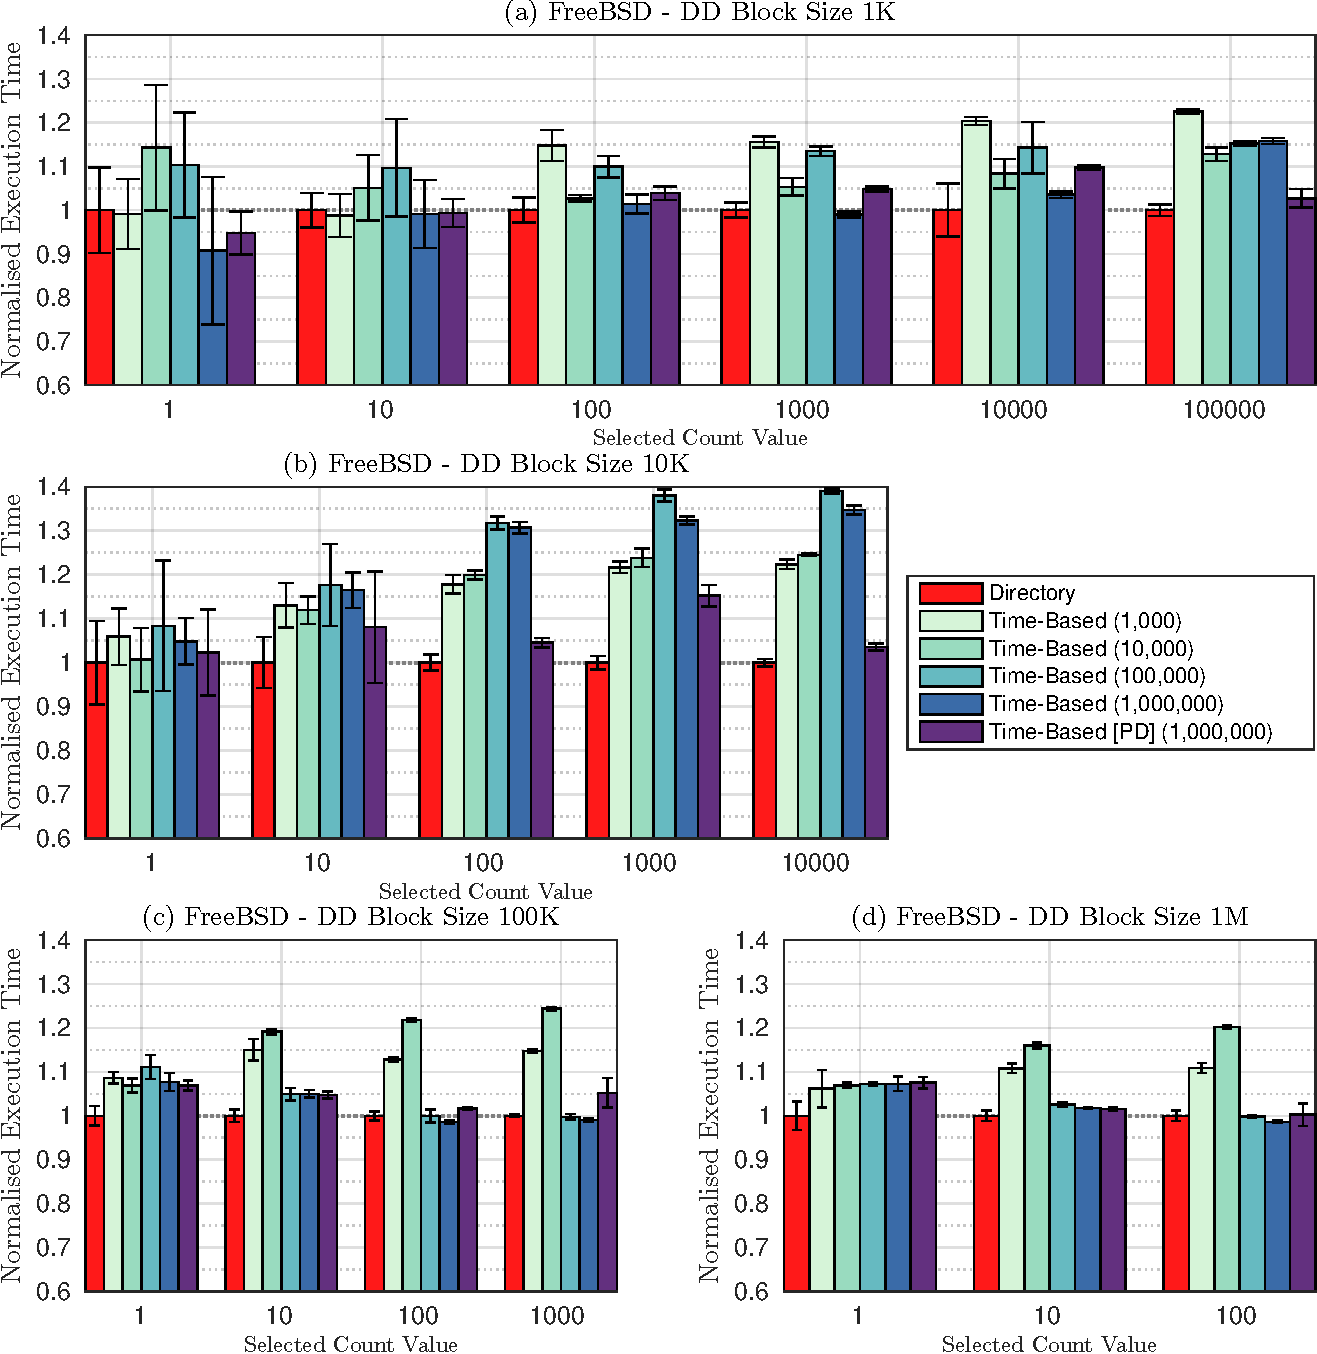
\includegraphics[width=\textwidth,height=\textheight,keepaspectratio,angle=0]{dd_freebsd_full}}
			\caption{FreeBSD DD performance evaluation} 
			\label{dd_freebsd_full}
		\end{figure}
		
		The results (Figure \ref{dd_freebsd_full}) show that there is no distinct pattern between the time-based models across all test variants. However, for a given block size the behaviour is somewhat consistent. The PD scheme is consistent throughout the range, falling within 10\% of the directory execution time in all but one test.
		
		In test (a), all time-based models fall within 20\% of the baseline, with the standard (1,000,000) model performing better than PD in most cases. In test (b), the PD version is more consistent in its execution time and shows the best overall performance. Similar behaviour is observed in tests (c) and (d). 



%\clearpage	
	\subsection{CP}
		\label{results_cp}
		The file copy (cp) command is similar to (dd), however, it offers a higher level of abstraction and deals with files and directories rather than disk blocks. The test crafted based on the (cp) command deals with a fixed set of files ($\sim$100K, $\sim$1M and, $\sim$2M) and copies them between directories. The test performance is measured using hardware registers.
		
		\begin{figure}[!ht]
		\centering 
			\makebox{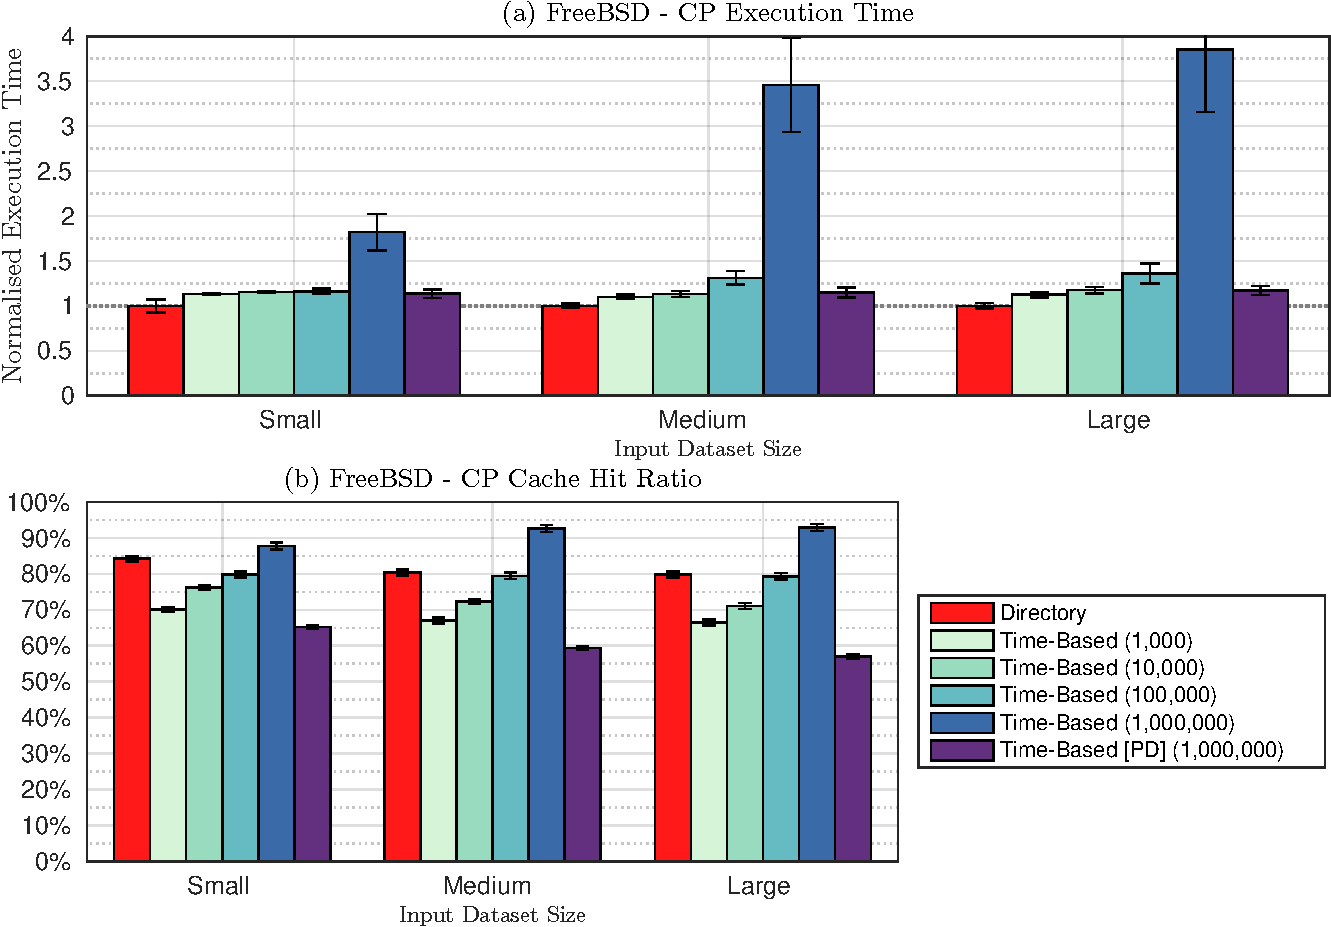
\includegraphics[width=\textwidth,height=\textheight,keepaspectratio,angle=0]{cp_freebsd_full}}
			\caption{FreeBSD CP performance evaluation} 
			\label{cp_freebsd_full}
		\end{figure}
		
		This application actively uses SYNC instructions, however, it still relies on memory polling. It is particularly evident from the exponential increase in execution time when comparing the 100,000 and 1,000,000 time-based models. The increasing standard deviation of the 1,000,000 model also suggests that some time-outs occur at favourable synchronisation boundaries, yielding a better execution time. This test was the primary cause for developing the hardware polling detection mechanism in the L1 data caches.
		
		Note the relatively low hit rate of the PD mechanism as compared to other schemes. In this experiment a higher miss rate in the time-based scheme is actually a positive indicator. It demonstrates that actively polled lines are refreshed. The directory uses coherence messages to update stale data, therefore it can retain the benefits of a higher hit rate. Also note that the standard 1,000,000 shows by far the best hit rate ($\sim$90\%), but also the worst performance. The directory hit rate actually reduces with the increase in test size; the same is true for the PD model.
		
		
	\subsection{GREP}
		\label{results_grep}
		The grep command is used for searching plaint-text data and matching a regular expression. The algorithm used by grep is very efficient and allows fast searching of patterns. The test based on grep, searches a large text file for 3 distinct patterns. The selected patterns appear with varying frequency and quantity in the file, ranging from highly infrequent to highly frequent.

		\begin{figure}[!ht]
		\centering 
			\makebox{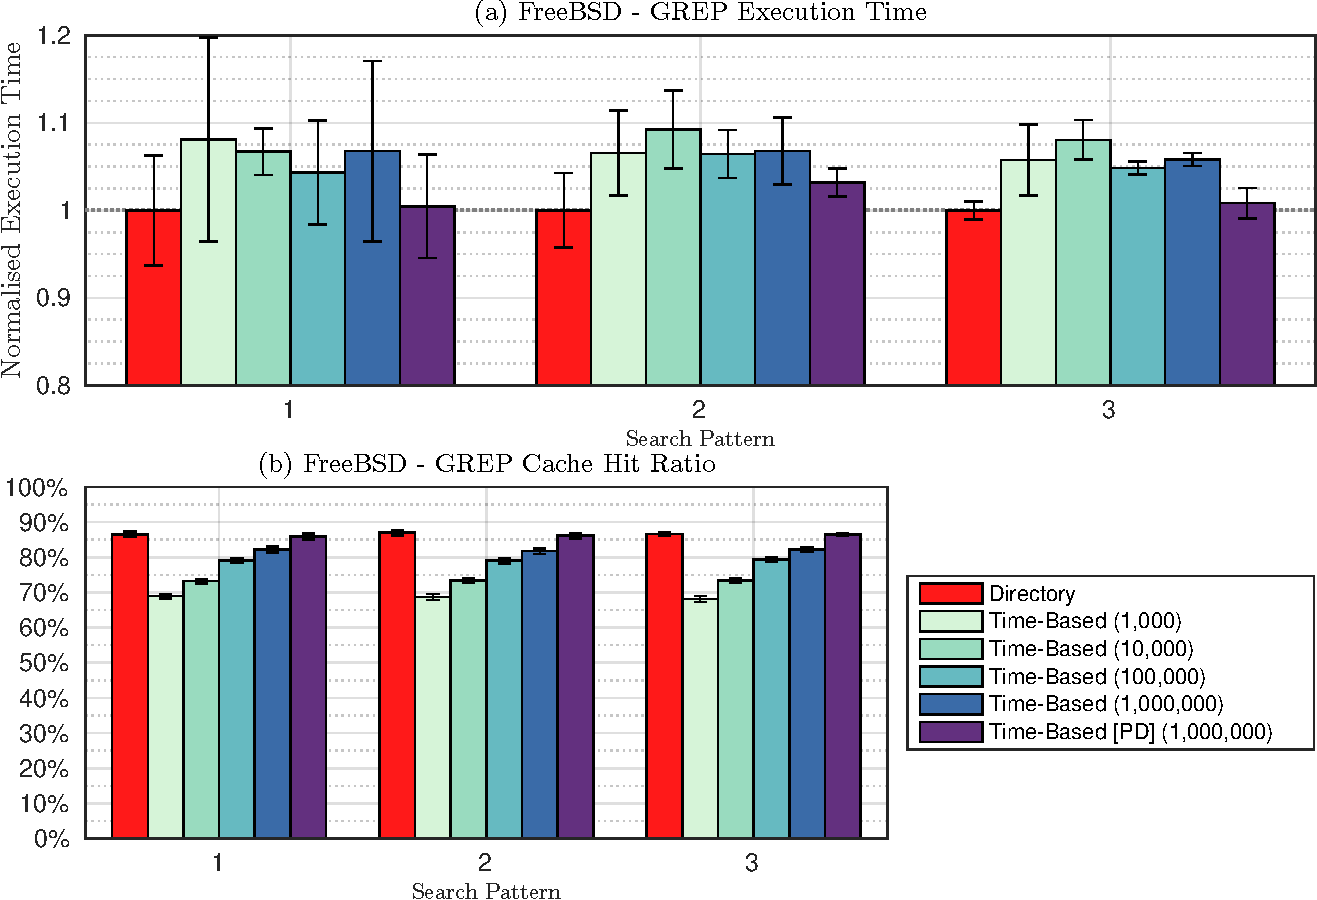
\includegraphics[width=\textwidth,height=\textheight,keepaspectratio,angle=0]{grep_freebsd_full}}
			\caption{FreeBSD GREP performance evaluation} 
			\label{grep_freebsd_full}
		\end{figure}

		The results are shown in Figure \ref{grep_freebsd_full}. The patterns are arranged in order of most frequent to least frequent. The PD model is the best performing time-based design. The execution time of all models is proportional to the individual hit ratios. The PD model achieves cache hit ratios closest to the directory, showing comparable performance. The standard deviation of the hit ratios is very low, indicating that any fluctuation in other time-based schemes is caused by OS or hardware behaviour. The variation in grep search patterns only affects the standard deviation of results and the relative performance of all coherence models is similar for every search pattern.
		

%\clearpage	
	\subsection{MD5}
		\label{results_md5}
		This widely adapted cryptographic hash function is commonly used to verify data integrity. The algorithm operates on variable sized data and generates a fixed length hash (128 bits). The input data is split into 512 bit blocks and padded when necessary. The algorithm consists of Boolean and memory operations. Time taken to produce the hash is proportional to the size of input data. Three files are used as input in this test, same as those used in the CP test.
		
		Test results are shown in Figure \ref{md5_freebsd_full}. The most performance variation is observed when hashing the smallest file size. For the time-based models (1,000 -- 100,000) the pattern is very similar, gradual execution time improvement. 
		
		\begin{figure}[!ht]
		\centering 
			\makebox{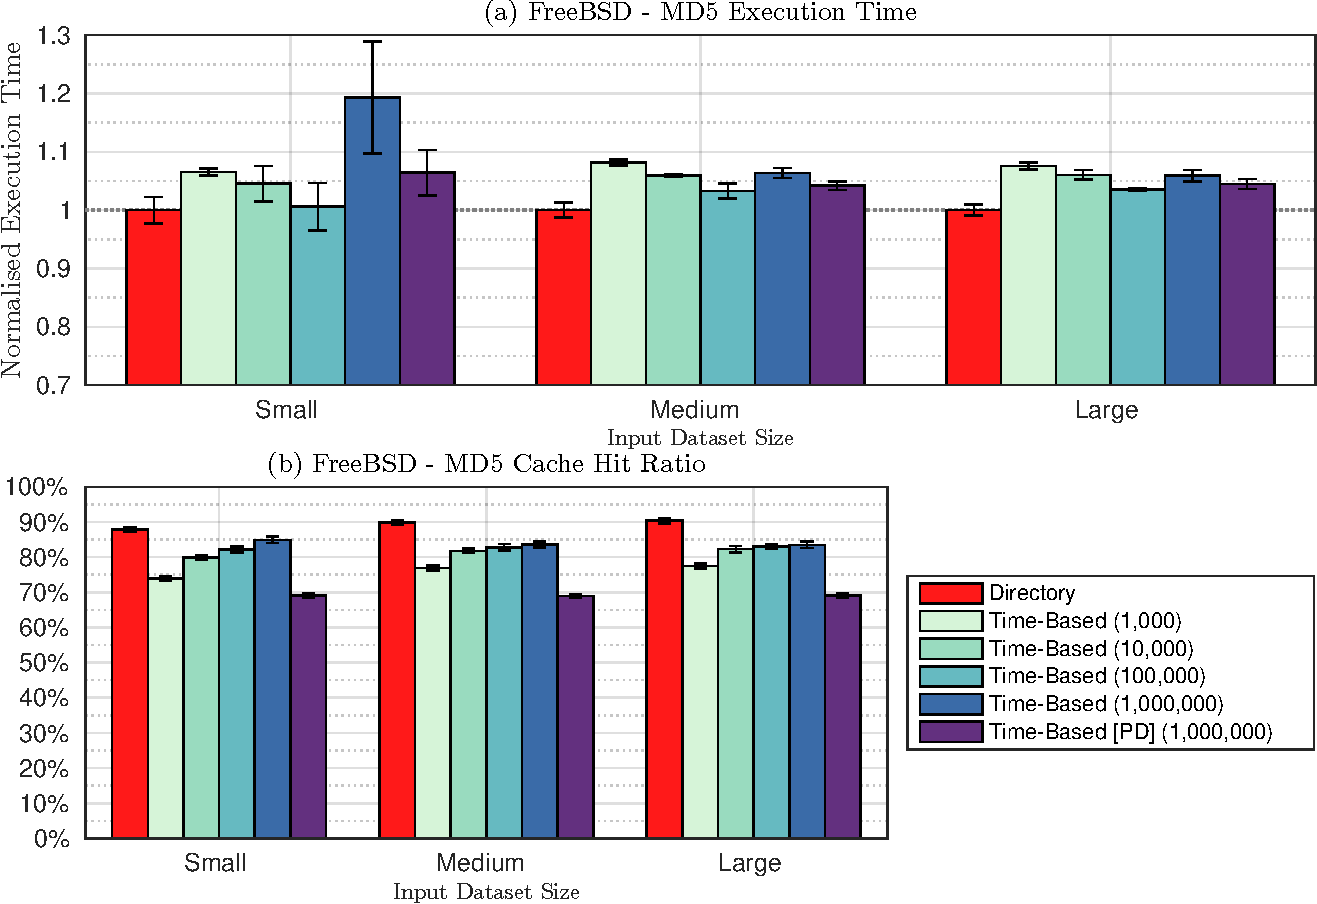
\includegraphics[width=\textwidth,height=\textheight,keepaspectratio,angle=0]{md5_freebsd_full}}
			\caption{FreeBSD MD5 performance evaluation} 
			\label{md5_freebsd_full}
		\end{figure}
		
		On an average the PD model is only second to the 100,000 model, despite showing the lowest hit rate. This indicates that some polling operations are used, and explains the sharp drop in performance from the 100,000 to 1,000,000 models. Note that polling operations are not inherent to the application itself, instead they are likely induced by the kernel when it schedules threads, services interrupts, and performs other functions.

			
%\clearpage	
	\subsection{SHA-256}
		\label{results_sha}
		This application is a common cryptographic hash function. As the name suggests, sha-256 yields 256 bit digests. The algorithm consists of Boolean and memory operations, performing multiple rounds on data blocks. Three input files are used, identical to previous tests.
		
		Test results are shown in Figure \ref{sha_freebsd_full}. In this test the PD scheme shows the weakest performance of all evaluated time-based models. The lower hit ratio of this model suggests that polling is being detected, however, the slow execution time suggests some false polling detection. The overall performance of the PD model is still within 10\% of the baseline. This test illustrates that the polling detection mechanism can be improved to limit false detection.

		\begin{figure}[!ht]
		\centering 
			\makebox{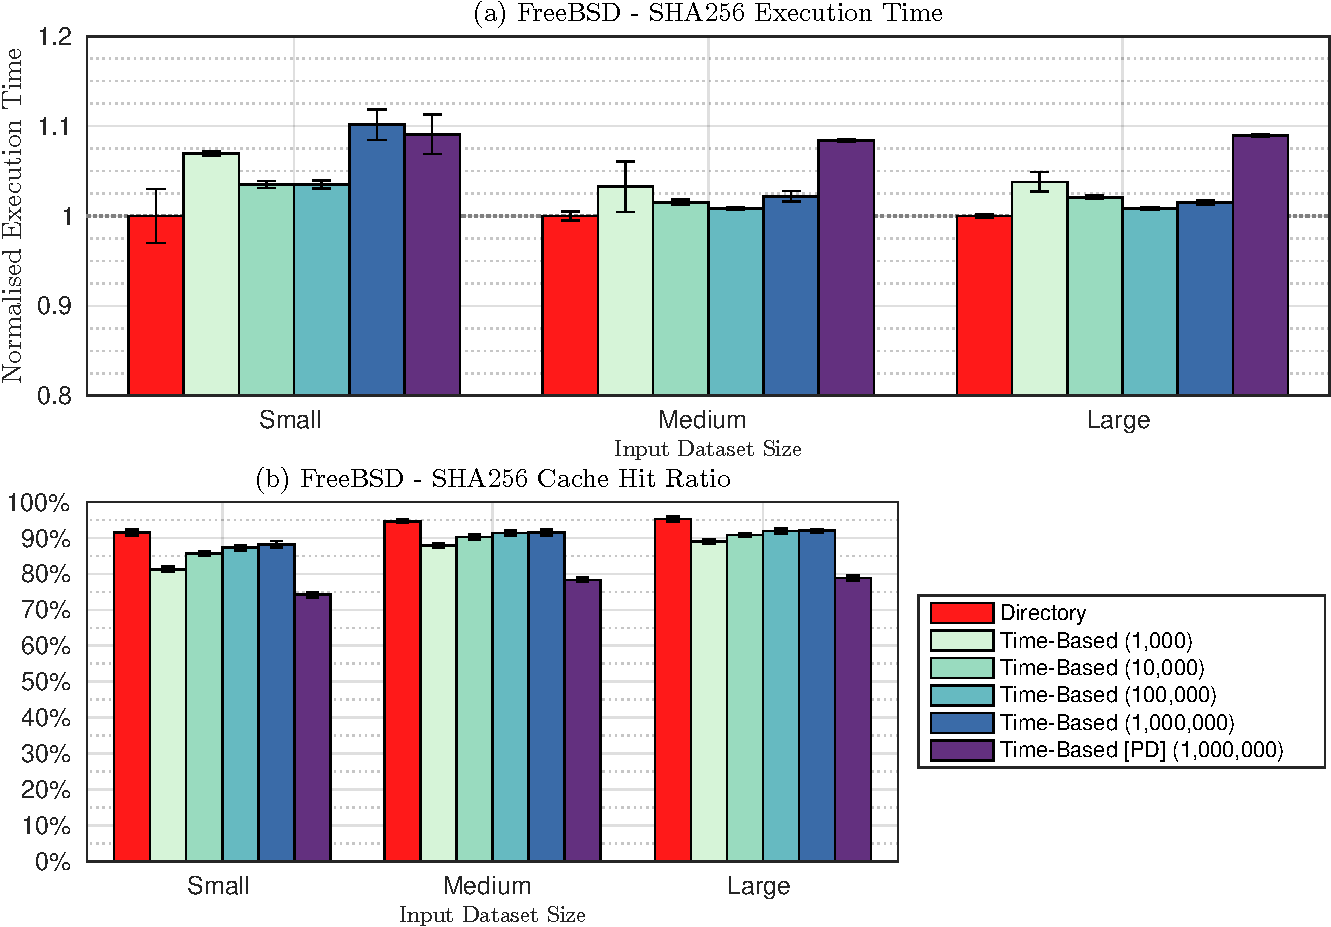
\includegraphics[width=\textwidth,height=\textheight,keepaspectratio,angle=0]{sha_freebsd_full}}
			\caption{FreeBSD SHA-256 performance evaluation} 
			\label{sha_freebsd_full}
		\end{figure}

%\clearpage
	\section{Communication Energy Estimation}
		The time-based coherence model does not require a coherence network, as a result the logic overheads are lower (elaborated in Section \ref{section_fpga_overheads}). However, results discussed in this chapter show that this coherence mechanism frequently increases the cache miss rate, generating more memory requests than the directory mechanism. 
		
		Cache statistics collected for the Splash-2 benchmarks can be used to calculate the communication overheads between the L1 and L2 caches for both coherence schemes. The bit lengths of memory requests and coherence messages is known, thus, energy can be estimated in terms of the number of bits communicated.
	
		\subsection{Parallel Execution}
			The BERI L1 data cache is non-write allocate and cache lines are only updated on load misses. The number of essential bits required for each type of memory request are listed below:
			\begin{itemize}
				\item L1 data cache fill request: physical address (physically mapped L2) + transaction ID (merge unit distinguishes between requests from different cores) + cached + linked (LL) $\Rightarrow$ \{40 + 8 + 1 + 1\} $\Rightarrow$ 50 bits.
				\item L2 fill response: data + transaction ID $\Rightarrow$ \{256 + 8\} $\Rightarrow$ 264 bits.
				\item Coherence message: subset of physical address (short tags do not require full address) + sharers list (core count relative) $\Rightarrow$ \{24 + 2\} $\Rightarrow$ 26 bits.
			\end{itemize}
			
			The energy cost of a cache miss is a sum of the fill request and fill response (50 + 264 = 314 bits) multiplied by the energy expended for transferring 1 bit. I will assume that the cost per bit is constant for BERI coherence models, as they use the same network. I will also assume that the energy cost for each bit of a coherence message is the same as that of a fill message. While the coherence network is separate, it runs in parallel to the regular memory network.
			
			\begin{description}
				\item [Directory-based coherence] In order to calculate communication energy overheads, the total number of cache read misses and coherence messages per test are counted. These two values allow us to estimate the total communication energy: total read miss cost + total coherence message cost.
				\item [Time-based coherence] The energy cost for this mechanism is simply the cost of a read miss. In this evaluation, I have used the time-based (1,000,000) model with no polling detection. The detector has been omitted as it is not integral to the coherence scheme.
			\end{description}

			The total communication between the L1 and L2 caches for the Splash-2 benchmarks previously used reveals that the energy consumption of the time-based scheme is within $\pm$1\% of the directory baseline value. Note that this result represents a combined total of all relevant communication displayed by the 11 benchmarks. The communication costs are obtained for 2 and 16 software thread test variants.
			The memory usage of each benchmark is different, hence, the total energy overhead displayed here is not representative of individual test results.
			
			The two coherence models show greater variance for individual Splash-2 benchmarks. For instance, in the FMM (Small) test, the time-based model shows a significant overhead of $\sim$16--22\%. However, when evaluated with the FMM (Large) test, the coherence model requires $\sim$2--4\% less energy than the directory. The performance of the time-based coherence improves with an increase in dataset size, thus the energy overheads are also lower.
			
			Prior evaluation has shown that the time-based model shows a weak relative performance for the Radix benchmark. The energy evaluation shows that the time-based model requires $\sim$32--50\% more energy than the directory.
			
			The time-based model does not display the best performance in the LU Contiguous benchmark, however, it shows a much better hit rate and requires 29--36\% less energy than the directory design. The directory actively communicates with all sharers, producing a better overall performance at the cost of energy overheads.
			
			These results show a large variation in communication overheads which is expected due to the diverse benchmark behaviour. The Radix benchmark manipulates local histograms and requires more fine-grained communication, which results in performance and energy overheads. The LU Contiguous benchmark is evaluated using a large block size which is much better suited to the time-based model. The FMM Small and Large tests show that for the same benchmark, significant energy and performance variations may be observed due to memory sharing patterns.
			
			The time-based model suffers overheads due to the high cost of memory fetch operations. Every fetch costs 314 bits which is approximately 12 times more than the cost of a single coherence message. The time-based model shows a good average hit ratio but it is lower than that shown by the directory. If the cost of the coherence message is increased and all other hardware parameters are unchanged, the time-based model could be more energy efficient.
			
			Note that the energy estimates presented here only focus on L1--L2 communication traffic and do not account for other variables. For instance, the directory model will expend energy through additional sharer bit lookups, coherence interface, memory controller, L1 cache coherence interface, and L1 invalidation logic. The time-based model energy expenditure will include the TTS, time-counters, and SYNC logic.
			
		\subsection{Independent Concurrent Execution}
			Multiple independent applications do not explicitly share any data, however, they do share cache space. Since cache space is limited, the applications may cause false sharing or cache thrashing. These effects are usually reduced by using associative caches. However, if the memory usage of one or both applications is high, it is likely that they will replace each other data in the caches due to cache capacity misses. 
			
			The BERI directory-based coherence mechanism is strictly inclusive and this is a disadvantage when it comes to independent applications, since the directory will need to send a coherence message to any sharer cache upon data eviction. This will result in coherence traffic and cache blocking overheads. 
			
			The time-based scheme is not influenced by shared memory evictions so it has an advantage over the directory-based scheme. The time-based model will still suffer penalties due to automatic self-invalidation and SYNC based self-invalidation, but these overheads are likely to be lower than those faced by the directory model.

		
	\section{Scalability Estimation}
		In this section I look at the current storage overheads of the BERI coherence schemes and extrapolate them to a larger number of cores.
		
		\subsection{Directory-based coherence}
			The storage overheads for this model have already been discussed in Sections \ref{dir_data_cache_structure} and \ref{dir_llc_structure}. I do not currently send any coherence messages to the L1 instruction caches so there are no overheads for these. The L1 data caches have a fixed overhead due to the short-tags optimisation, used to speed up invalidations. 
			
			In the L2 cache the directory sharers list requires one bit per cache line per L1 data cache. Thus, the directory shows a linear overhead for the sharers list. If the L1 instruction cache accesses need to be tracked then the overheads will double but would then remain constant. 
			
			The BERI caches use a fixed line capacity of 32 bytes. If you were to connect 256 L1 data caches into this L2 cache, the directory overheads per cache line would be equal to the data size (100\%). This is a highly unreasonable scenario, and beyond 4--16 cores we would expect a multiple level hierarchy such as the one outlined by Martin et al. \cite{Martin12}. The authors show that a three-level scheme can significantly improve directory overheads, less than 2\% for 256 cores. 
		
		\subsection{Time-based coherence}
			This coherence model does not add any overheads to shared memory since all of the logic is held within the L1 data caches. As with the directory design, the time-based model is not applied to the L1 instruction caches. The L1 data cache structure has been discussed in Section \ref{tts_memory_overhead}. 
			
			The tag-time-stamp adds a fixed overhead to each cache line, 4 bits in the current version. The TTS is variable and could be optimised to use smaller sizes in future versions of the coherence protocol. Darnell and Kennedy \cite{Darnell93} have previously demonstrated a timestamp based coherence mechanism which only requires 1 bit per cache line.
			
			Attaching multiple L1 data caches to a single shared memory will not add any coherence overheads to the memory infrastructure, however, larger designs would require a multi-level design, such as the one described for directory-coherence above. The time-based model implemented in the L1 caches can be extended to the L2 cache and beyond. A fixed overhead will be added to each cache line in the multiple L2's.

		
	\section{Simplicity}
		It is difficult to quantify the simplicity of a cache coherence mechanism as some estimates may be subjective. From a hardware standpoint, the simplest coherence mechanism is one that relies purely on software support, but software developers prefer a less complex model.
		
		The directory-based coherence scheme requires more infrastructure and resources as compared to the time-based model. The directory must track sharer caches and distribute coherence messages, whereas the time-based coherence scheme need not be aware of any other caches.
		
		Hardware overheads are another way of judging design complexity. I have already illustrated the FPGA overheads for both coherence schemes (Section \ref{section_fpga_overheads}), and the time-based scheme requires 1--2\% less logic. FPGA logic and area overheads are variable and HDL optimisations may change the final design outcome. I have to trust the Bluespec compiler and Quartus tools to make correct optimisations.
		
		Development time is also a factor worth considering, however, it is highly subjective. I required more time to develop the BERI directory protocol and adapt it for FreeBSD OS support, however, unanticipated hardware and OS bugs extended the development time. Whereas, the first iteration of the time-based protocol was able to boot the OS and remained stable throughout.

%\clearpage
	\section{Summary}
		The evaluation of the time-based model has shown that it is possible to approach the performance level of directory-based coherence without any explicit messaging. The polling detection optimisation significantly improves the time-based protocol. However, the directory-based coherence design is undoubtedly superior over a wide range of test variations, moreover the benefits of coherence messaging are evident. 
		
		Future improvements and optimisations of the time-based protocol could allow this scheme to surpass the performance of level of this directory-based design. The two protocols have been evaluated on a dual-core system, and a larger system behaviour is yet unknown.
